\documentclass[man]{apa6}
\usepackage{lmodern}
\usepackage{amssymb,amsmath}
\usepackage{ifxetex,ifluatex}
\usepackage{fixltx2e} % provides \textsubscript
\ifnum 0\ifxetex 1\fi\ifluatex 1\fi=0 % if pdftex
  \usepackage[T1]{fontenc}
  \usepackage[utf8]{inputenc}
\else % if luatex or xelatex
  \ifxetex
    \usepackage{mathspec}
  \else
    \usepackage{fontspec}
  \fi
  \defaultfontfeatures{Ligatures=TeX,Scale=MatchLowercase}
\fi
% use upquote if available, for straight quotes in verbatim environments
\IfFileExists{upquote.sty}{\usepackage{upquote}}{}
% use microtype if available
\IfFileExists{microtype.sty}{%
\usepackage{microtype}
\UseMicrotypeSet[protrusion]{basicmath} % disable protrusion for tt fonts
}{}
\usepackage{hyperref}
\hypersetup{unicode=true,
            pdftitle={The development of infants' responses to mispronunciations: A Meta-Analysis},
            pdfauthor={Katie Von Holzen~\& Christina Bergmann},
            pdfkeywords={language acquisition; mispronunciation sensitivity; word recognition;
meta-analysis; lexicon; infancy},
            pdfborder={0 0 0},
            breaklinks=true}
\urlstyle{same}  % don't use monospace font for urls
\usepackage{graphicx,grffile}
\makeatletter
\def\maxwidth{\ifdim\Gin@nat@width>\linewidth\linewidth\else\Gin@nat@width\fi}
\def\maxheight{\ifdim\Gin@nat@height>\textheight\textheight\else\Gin@nat@height\fi}
\makeatother
% Scale images if necessary, so that they will not overflow the page
% margins by default, and it is still possible to overwrite the defaults
% using explicit options in \includegraphics[width, height, ...]{}
\setkeys{Gin}{width=\maxwidth,height=\maxheight,keepaspectratio}
\IfFileExists{parskip.sty}{%
\usepackage{parskip}
}{% else
\setlength{\parindent}{0pt}
\setlength{\parskip}{6pt plus 2pt minus 1pt}
}
\setlength{\emergencystretch}{3em}  % prevent overfull lines
\providecommand{\tightlist}{%
  \setlength{\itemsep}{0pt}\setlength{\parskip}{0pt}}
\setcounter{secnumdepth}{0}
% Redefines (sub)paragraphs to behave more like sections
\ifx\paragraph\undefined\else
\let\oldparagraph\paragraph
\renewcommand{\paragraph}[1]{\oldparagraph{#1}\mbox{}}
\fi
\ifx\subparagraph\undefined\else
\let\oldsubparagraph\subparagraph
\renewcommand{\subparagraph}[1]{\oldsubparagraph{#1}\mbox{}}
\fi

%%% Use protect on footnotes to avoid problems with footnotes in titles
\let\rmarkdownfootnote\footnote%
\def\footnote{\protect\rmarkdownfootnote}


  \title{The development of infants' responses to mispronunciations: A
Meta-Analysis}
    \author{Katie Von Holzen\textsuperscript{1,2}~\& Christina
Bergmann\textsuperscript{3,4}}
    \date{}
  
\shorttitle{Mispronunciation Meta-Analysis}
\affiliation{
\vspace{0.5cm}
\textsuperscript{1} Department of Hearing and Speech Sciences, University of Maryland, USA\\\textsuperscript{2} Laboratoire Psychologie de la Perception, Université Paris Descartes\\\textsuperscript{3} Max Planck Institute for Psycholinguistics, Nijmegen, the Netherlands\\\textsuperscript{4} LSCP, Departement d'Etudes Cognitives, ENS, EHESS, CNRS, PSL Research University}
\keywords{language acquisition; mispronunciation sensitivity; word recognition; meta-analysis; lexicon; infancy}
\usepackage{csquotes}
\usepackage{upgreek}
\captionsetup{font=singlespacing,justification=justified}

\usepackage{longtable}
\usepackage{lscape}
\usepackage{multirow}
\usepackage{tabularx}
\usepackage[flushleft]{threeparttable}
\usepackage{threeparttablex}

\newenvironment{lltable}{\begin{landscape}\begin{center}\begin{ThreePartTable}}{\end{ThreePartTable}\end{center}\end{landscape}}

\makeatletter
\newcommand\LastLTentrywidth{1em}
\newlength\longtablewidth
\setlength{\longtablewidth}{1in}
\newcommand{\getlongtablewidth}{\begingroup \ifcsname LT@\roman{LT@tables}\endcsname \global\longtablewidth=0pt \renewcommand{\LT@entry}[2]{\global\advance\longtablewidth by ##2\relax\gdef\LastLTentrywidth{##2}}\@nameuse{LT@\roman{LT@tables}} \fi \endgroup}


\DeclareDelayedFloatFlavor{ThreePartTable}{table}
\DeclareDelayedFloatFlavor{lltable}{table}
\DeclareDelayedFloatFlavor*{longtable}{table}
\makeatletter
\renewcommand{\efloat@iwrite}[1]{\immediate\expandafter\protected@write\csname efloat@post#1\endcsname{}}
\makeatother
\usepackage{lineno}

\linenumbers
\usepackage{setspace}
\AtBeginEnvironment{tabular}{\singlespacing}
\AtBeginEnvironment{lltable}{\singlespacing}
\AtBeginEnvironment{tablenotes}{\doublespacing}
\captionsetup[table]{font={stretch=1.5}}
\captionsetup[figure]{font={stretch=1.5}}

\authornote{The authors each declare that they have no
conflict of interest.

Correspondence concerning this article should be addressed to Katie Von
Holzen, 0221A LeFrak Hall, University of Maryland, College Park, MD
20742. E-mail:
\href{mailto:katie.m.vonholzen@gmail.com}{\nolinkurl{katie.m.vonholzen@gmail.com}}}

\abstract{
As they develop into mature speakers of their native language, infants
must not only learn words but also the sounds that make up those words.
To do so, they must strike a balance between accepting some variation
(e.g.~mood, voice, accent), but appropriately rejecting variation when
it changes a word's meaning (e.g.~cat vs.~hat). We focus on studies
investigating infants' ability to detect mispronunciations in familiar
words, which we refer to as mispronunciation sensitivity. The goal of
this meta-analysis was to evaluate the development of mispronunciation
sensitivity in infancy, allowing for a test of competing mainstream
theoretical frameworks. The results show that although infants are
sensitive to mispronunciations, they still accept these altered forms as
labels for target objects. Interestingly, this ability is not modulated
by age or vocabulary size, challenging existing theories and suggesting
that a mature understanding of native language phonology is present in
infants from an early age, possibly before the vocabulary explosion.
Despite this finding, we discuss potential data analysis choices that
may influence different conclusions about mispronunciation sensitivity
development as well as offer recommendations to improve best practices
in the study of mispronunciation sensitivity.


}

\usepackage{amsthm}
\newtheorem{theorem}{Theorem}[section]
\newtheorem{lemma}{Lemma}[section]
\theoremstyle{definition}
\newtheorem{definition}{Definition}[section]
\newtheorem{corollary}{Corollary}[section]
\newtheorem{proposition}{Proposition}[section]
\theoremstyle{definition}
\newtheorem{example}{Example}[section]
\theoremstyle{definition}
\newtheorem{exercise}{Exercise}[section]
\theoremstyle{remark}
\newtheorem*{remark}{Remark}
\newtheorem*{solution}{Solution}
\begin{document}
\maketitle

\section{Introduction}\label{introduction}

At the turn of the millenium, infant language acquisition researchers
had established that during their first two years of life, infants are
sensitive to changes in the phonetic detail of newly segmented words
(Jusczyk \& Aslin, 1995) and learned minimal pairs (Stager \& Werker,
1997). Furthermore, when presented with familiar image pairs, children
fixate on the referent of a spoken label (Fernald, Pinto, Swingley,
Weinberg, \& McRoberts, 1998; Tincoff \& Jusczyk, 1999). Swingley and
Aslin (2000) were the first to tie these lines of research together and
investigate mispronunciation sensitivity in infant familiar word
recognition: Children aged 18 to 23 months learning American English saw
pairs of images (e.g.~a baby and a dog) and their eye movements to each
image were recorded. On \enquote{correct} trials, children heard the
correct label for one of the images (e.g. \enquote{baby}). On
\enquote{mispronounced} trials, children heard a mispronounced label of
one of the images (e.g. \enquote{vaby}). The mean proportion of
fixations to the target image (here: a baby) was calculated separately
for both correct and mispronounced trials by dividing the target looking
time by the sum of total looking time to both target and a distractor
(proportion of target looking or PTL). Mean fixations in correct trials
were significantly greater than in mispronounced trials, and in both
conditions looks to the target were significantly greater than chance.
We refer to this pattern of a difference between looks to correct and
mispronounced words as \emph{mispronunciation sensitivity} and of looks
to the target image above chance in each condition as \emph{object
identification}. Swingley and Aslin (2000) concluded that already before
the second birthday, children represent words with sufficient detail to
be sensitive to mispronunciations.

In a mature phono-lexical system, word recognition must balance
flexibility to slight variation (e.g., speaker identity, accented
speech) while distinguishing between phonological contrasts that
differentiate words in a given language (e.g.~cat-hat). The study of
Swingley and Aslin (2000) as well as subsequent studies examining
mispronunciation sensitivity probe this latter distinction. Phonological
contrasts relevant for the infant language-learner are determined by
their native language. For an infant learning Catalan, the vowel
contrast /e/-/E/ signifies a change in meaning, whereas this is not the
case for an infant learning Spanish. These contrasts are therefore not
inate, but must be learned. In this meta-analysis, we focus on infants'
developing ability to correctly apply the phonological distinctions for
their native language during word recognition. By aggregating all
publicly available evidence using meta-analysis, we can examine
developmental trends making use of data from a much larger and diverse
sample of infants than is possible in most single studies (see Frank et
al. (2017); for a notable exception). Before we outline the
meta-analytical approach and its advantages in detail, we first discuss
the proposals this study seeks to disentangle and the data supporting
each of the accounts.

Research following the seminal study by Swingley and Aslin (2000) has
extended mispronunciation sensitivity to infants as young as 8 to 10
months (Bergelson \& Swingley, 2017), indicating that from early stages
of the developing lexicon onwards, infants can and do detect
mispronunciations. Regarding the change in mispronunciation sensitivity
over development, however, only about half of studies have compared more
than one age group on the same mispronunciation task (see Table 1).
Across single studies all possible patterns of development lined out
above have been reported, making the current meta-analysis very
informative.

Several studies have found evidence for \emph{greater} mispronunciation
sensitivity as children develop. More precisely, the difference in
target looking for correct and mispronounced trials is reported to be
smaller in younger infants and grows as infants develop. Mani and
Plunkett (2007) tested 15-, 18-, and 24-month-olds learning British
English; although all three groups were sensitive to mispronunciations,
15-month-olds showed a less robust sensitivity. An increase in
sensitivity to mispronunciations has also been found from 20 to 24
months (Feest \& Fikkert, 2015) and 15 to 18 months (Altvater-Mackensen,
Feest, \& Fikkert, 2014) in Dutch infants, as well as German infants
from 22 to 25 months (Altvater-Mackensen, 2010). Furthermore, Feest and
Fikkert (2015) found that sensitivity to specific kinds of
mispronunciations develop at different ages depending on language
infants are learning. In other words, the native language constraints
which \emph{kinds} of mispronunciations infants are sensitive to first,
and that as infants develop, they become sensitive to other
mispronunciations.

Other studies have found no difference in mispronunciation sensitivity
at different ages. For example, Swingley and Aslin (2000) tested infants
over a wide age range of 5 months (18 to 23 months). They found that age
correlated with target fixations for both correct and mispronounced
labels, whereas the difference between the two (mispronunciation
sensitivity) did not. This suggests that as children develop, they are
more likely to look at the target in the presence of a correct or
mispronounced label, but that the difference between looks elicited by
the two conditions does not change. A similar response pattern has been
found for British English learning infants aged between 18 and 24 months
(Bailey \& Plunkett, 2002) as well as younger French-learning infants at
12 and 17 months (Zesiger, Lozeron, Levy, \& Frauenfelder, 2012).

One study has found evidence for infants to become \emph{less} sensitive
to mispronunciations as they develop. Mani and Plunkett (2011) presented
18- and 24-month-olds with mispronunciations varying in the number of
phonological features changed (e.g., changing an p into a b, a 1-feature
change, versus changing a p into a g, a 2-feature change). 18-month-olds
were sensitive to mispronunciations, regardless of the number of
features changed. 24-month-olds, in contrast, fixated the target image
equally for both correct and 1-feature mispronounced trials, although
they were sensitive to larger mispronunciations. In other words, for
1-feature mispronunciations at least, sensitivity decreased from 18 to
24 months.

Why would mispronunciation sensitivity change as infants develop?
Typically, a change in mispronunciation sensitivity is thought to occur
along with an increase in vocabulary size, particularly with the
vocabulary spurt at about 18 months. As infants learn more words, their
focus shifts to the relevant phonetic dimensions needed for word
recognition. For example, an infant who knows a handful of words with
few phonological neighbors would not need to have fully specified
phonological representations in order to differentiate between these
words. As more phonologically similar words are learned, however, the
need for fully detailed phonological representations increases
(Charles-Luce \& Luce, 1995). Furthermore, a growing vocabulary also
reflects increased experience or familiarity with words, which may
sharpen the detail of their phonological representation (Barton, Miller,
\& Macken, 1980). If vocabulary growth leads to an increase in the
phonological specificity of infants' word representation, we should find
a relationship between vocabulary size and mispronunciation sensitivity.

Yet, the majority of studies examining a potential association between
mispronunciation sensitivity and vocabulary size have concluded that
there is no relationship (Bailey \& Plunkett, 2002; Ballem \& Plunkett,
2005; Mani \& Plunkett, 2007; Mani, Coleman, \& Plunkett, 2008;
Swingley, 2009; Swingley \& Aslin, 2000, 2002; Zesiger et al., 2012).
One notable exception comes from Mani and Plunkett (2010). Here,
12-month-old infants were divided into a low and high vocabulary group
based on median vocabulary size. High vocabulary infants showed greater
sensitivity to vowel mispronunciations than low vocabulary infants,
although this was not the case for consonant mispronunciations. Taken
together, there is very little evidence for a role of vocabulary size in
mispronunciation sensitivity. In our current meta-analysis, we include
the relationship between mispronunciation sensitivity and vocabulary
size to better understand the variation in experimental results.

Although all mispronunciation sensitivity studies are generally
interested in the the phonological detail with which infants represent
familiar words, many studies pose more nuanced questions. These
questions concern issues at the intersection of phonological development
and lexical processing and often result in manipulations of the stimuli
and experimental procedure. Next to the core investigation of the shape
of development of infants' mispronunciation sensitivity, we take the
opportunity of a systematic aggregation of data to address these
questions and the influence of these manipulations on infants' ability
to detect mispronunciations and how this may change with development.

In designing their mispronunciation stimuli, Swingley and Aslin (2000)
chose consonant mispronunciations that were likely to confuse adults
(Miller \& Nicely, 1955). Subsequent research has settled on
systematically modulating phonemic features to achieve mispronunciations
of familiar words. By utilizing mispronunciations consisting of phonemic
changes, these experiments examine infants' sensitivity to factors that
change the identity of a word on a measurable level (i.e.~1-feature,
2-features, 3-features, etc.). The importance of controlling for the
degree of phonological mismatch, as measured by number of features
changed, is further highlighted by studies that find graded sensitivity
to both consonant (White \& Morgan, 2008) and vowel (Mani \& Plunkett,
2011) feature changes. The greater the number of features changed, or
\emph{mispronunciation size}, the easier it may be to detect a
mispronunciation, whereas more similar mispronunciations may be more
difficult to detect.

Although most research examining sensitivity to mispronunciations
follows a similar design, there are some notable differences. For
example, Swingley and Aslin (2000) presented infants with pairs of
familiar images, one serving as the labeled target and one as the
unlabeled distractor. In contrast, White and Morgan (2008; see also Mani
\& Plunkett, 2011; Skoruppa et al., 2013; Swingley, 2016) presented
infants with pairs of familiar (labeled target) and unfamiliar
(unlabeled distractor) objects. By using an unfamiliar object as a
distractor, the infant is presented with a viable option onto which the
mispronounced label can be applied (Halberda, 2003; Markman, Wasow, \&
Hansen, 2003). Infants ages 24 and 30 months associate a novel label
with an unfamiliar object, although only 30-month-olds retained this
label-object pairing (Bion, Borovsky, and Fernald, 2013). In contrast,
18-month-olds did not learn to associate a novel label with an
unfamiliar object, providing evidence that this ability is developing
from 18 to 30 months. We may find that if mispronunciation sensitivity
changes as children develop, that this change is modulated by
\emph{distractor familiarity}: whether the distractor used is familiar
or unfamiliar. Although mispronunciation sensitivity in the presence of
a familiar compared to unfamiliar distractor has not been directly
compared, the baseline preference for familiar compared to novel stimuli
is also thought to change as infants develop (Hunter \& Ames, 1988).
Furthermore, young children have been found to look longer at objects
for which they know the name, compared to objects of an unknown name
(Schafer \& Plukett, 1998). In other words, in absentia of a label,
infants may be more or less likely to fixate on an unfamiliar object. To
account for inherent preferences to the target or distractor image,
mispronunciation experiments typically compare the increase in fixations
to the target image from a silent baseline to post-labeling or present
the same yoked pairs of target and distractor images in in both a
correct and mispronounced labelling context. Considering this evidence,
we may expect that in older, but not younger, children, the presence of
an unfamiliar distractor may lead to greater mispronunciation
sensitivity than in the presence of a familiar distractor.

Furthermore, when presenting infants with a familiar distractor image,
some studies control the \emph{phonological overlap between target and
distractor labels}. For example, when examining sensitivity to a
mispronunciation of the target word \enquote{dog}, the vowel
mispronunciation \enquote{dag} would be paired with a distractor image
that shares onset overlap, such as \enquote{duck}. This ensures that
infants can not use the onset of the word to differentiate between the
target and distractor images (Fernald, Swingley, \& Pinto, 2001).
Instead, infants must pay attention to the mispronounced phoneme in
order to successfully detect the change. The influence of distractor
overlap also depends on the \emph{position of mispronunciation} in the
word, which can be at word onset, medial, or final positions. Models of
spoken word processing place more or less importance on the position of
a phoneme in a word. The COHORT model (Marslen-Wilson \& Zwitserlood,
1989) describes lexical access in one direction, with the importance of
each phoneme decreasing as its position comes later in the word. In
contrast, the TRACE model (McClelland \& Elman, 1986) describes lexical
access as constantly updating and reevaluating the incoming speech input
in the search for the correct lexical entry, and therefore can recover
from word onset and to a lesser extent medial mispronunciations.

TRACE has also been used to model infants' sensitivity to
mispronunciation position (Mayor \& Plunkett, 2014), finding that as
lexicon size increases, so does sensitivity to onset mispronunciations,
whereas medial mispronunciations do not experience similar growth. In
early language acquisition, infants typically know more consonant
compared to vowel onset words. When tested on their recognition of
familiar words, therefore, younger infants would show greater
sensitivity to onset mispronunciations, which are frequently consonant
mispronunciations. The prevalence of consonant onset words may
contribute to the finding that consonants carry more weight in lexical
processing (C-bias; see Nazzi, Poltrock, \& Von Holzen, 2016 for a
recent review). In mispronunciation sensitivity, this would translate to
consonant mispronunciations impairing word recognition to a greater
degree than vowel mispronunciations. Yet, the handful of studies
directly comparing sensitivity to consonant and vowel mispronunciations
mostly find symmetry as opposed to an asymmetry between consonants and
vowels. English-learning 12-, 15-, 18-, and 24-month-olds (Mani \&
Plunkett, 2007; 2010 keps and tups) and Danish-learning 20-month-olds
(Hojen et al., unpublished) demonstrate similar sensitivity to consonant
and vowel mispronunciations. One study did find weak evidence for
greater sensitivity to consonant compared to vowel mispronunciations
(Swingley, 2016). The English-learning infants tested by Swingley were
older than previous studies (mean age 28 months). In word learning, the
C-bias has been found to develop later in English learning infants
(Floccia, Nazzi, Delle Luche, Poltrock, \& Goslin, 2014; Nazzi, Floccia,
Moquet, \& Butler, 2009). In the current meta-analysis, we attempt to
synthesize studies examining sensitivity to the \emph{type of
mispronunciation}, whether consonant or vowel, across different ages to
determine whether infants generally exhibit more sensitivity to
consonant compared to vowel mispronunciations in familiar word
recognition as predicted by a learned account of C-bias emergence
(Floccia et al., 2014; Keidel et al., 2007; Nazzi et al., 2016). We
further examine the impact of language family on mispronunciation
sensitivity to consonants and vowels, as C-bias emergence has been found
to have a different developmental trajectory for Romance (French,
Italian) compared to Germanic (British English, Danish) languages (Nazzi
et al., 2016).

Finally, mispronunciation sensitivity in infants has been examined in
many different languages, such as English, Spanish, French, Dutch,
German, Catalan, Danish, and Mandarin Chinese (see Table 1). Infants
learning different languages have different ages of acquisition for
words in their early lexicon, leaving direct comparisons between
languages within the same study difficult and as a result rare. Although
we do not explicitly compare overall mispronunciation sensitivity by
language (although see previous paragraph for rationale to test by
language family), we assess evidence of mispronunciation sensitivity
from many different languages using a meta-analytic approach.

In sum, the studies we have reviewed begin to paint a picture of the
development of infants' mispronunciation sensitivity. Each study
contributes one separate brushstroke and it is only by examining all of
them together that we can achieve a better understanding of the big
picture of early language development. Meta-analyses can provide unique
insights by estimating the population effect, both of infants' responses
to correct and mispronounced labels, and of their mispronunciations
sensitivity. Because we aggregate data over various age groups, this
meta-analysis can also investigate the role of maturation by assessing
the impact of age and vocabulary size. We also make hands-on
recommendations for experiment planning, for example by providing an
effect size estimate for a priori power analyses (Bergmann et al.,
2018).

\section{Methods}\label{methods}

The present meta-analysis was conducted with maximal transparency and
reproducibility in mind. To this end, we provide all data and analysis
scripts on the supplementary website (\url{https://osf.io/rvbjs/}) and
open our meta-analysis up for updates (Tsuji, Bergmann, \& Cristia,
2014). The most recent version is available via the website and the
interactive platform MetaLab (\url{https://metalab.stanford.edu};
Bergmann et al., 2018). Since the present paper was written with
embedded analysis scripts in R (R Core Team, 2018) using the papaja
package (Aust \& Barth, 2018) in R Markdown (Allaire et al., 2018), it
is always possible to re-analyze an updated dataset. In addition, we
followed the Preferred Reporting Items for Systematic Reviews and
Meta-Analyses (PRISMA) guidelines and make the corresponding information
available as supplementary materials (Moher, Liberati, Tetzlaff, Altman,
\& Group, 2009). Figure \ref{fig:PRISMA-image} plots our PRISMA
flowchart illustrating the paper selection procedure.

\subsection{(Insert Figure 1 about
here)}\label{insert-figure-1-about-here}

\begin{figure}
\centering
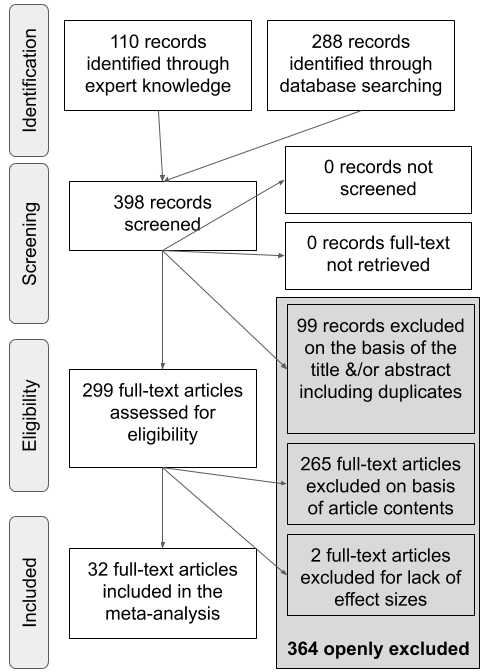
\includegraphics{figures/Figure_1_PRISMA_MA_Mispronunciation.png}
\caption{\label{fig:PRISMA-image}A PRISMA flowchart illustrating the
selection procedure used to include studies in the current
meta-analysis.}
\end{figure}

\subsection{Study Selection}\label{study-selection}

\begin{lltable}


\scriptsize{
\begin{longtable}{llllllllll}\noalign{\getlongtablewidth\global\LTcapwidth=\longtablewidth}
\caption{\label{tab:SummaryTable}Summary of all studies. Age: truncation of mean age reported in the paper. Vocabulary: Comp = comprehension, Prod = production. Distractor Familiarity: Fam = Familiar Distractor, Unfam = Unfamiliar Distractor. Distractor Target Overlap: position of overlap between target and distractor; O = onset, M = medial, C = coda. Mispronunciation Size: number of features changed; commas indicate when sizes were compared separately (e.g. 1, 2, 3), dashes indicate the range of sizes were aggregated (e.g. 1-3). Mispronunciation Position: O = onset, M = medial, C = coda. Mispronunciation Type: C = consonant, V = vowel, T = tone. For both Mispronunciation Position and Type, a slash separator indicates that is was tested but a distinction was not made in the stimuli. For all categories, unspec. indicates that the value was unspecified in the paper}\\
\toprule
 &  &  &  & \multicolumn{1}{c}{Distractor} & & \multicolumn{3}{c}{Mispronunciation}  &\\
\cmidrule(r){5-5} \cmidrule(r){7-9}
Paper & Format & Age & Vocabulary & Familiarity & Target Overlap & Size & Position & Type & N Effect Sizes\\
\midrule
Altvater-Mackensen (2010) & dissertation & 22, 25 & None & fam, unfam & O, novel & 1 & O, O/M & C & 13\\
Altvater-Mackensen et al. (2014) & paper & 18, 25 & None & fam & O & 1 & O & C & 16\\
Bailey \& Plunkett (2002) & paper & 18, 24 & Comp & fam & none & 1, 2 & O & C & 12\\
Bergelson \& Swingley (2017) & paper & 7, 9, 12, 6 & None & fam & none & unspec & O/M & V & 9\\
Bernier \& White (2017) & proceedings & 21 & None & unfam & novel & 1, 2, 3 & O & C & 4\\
Delle Luche et al. (2015) & paper & 20, 19 & None & fam & O & 1 & O & C/V & 4\\
Durrant et al. (2014) & paper & 19, 20 & None & fam & O & 1 & O & C/V & 4\\
Höhle et al. (2006) & paper & 18 & None & fam & none & 1 & O & C & 4\\
Højen et al. (n.d.) & gray paper & 19, 20 & Comp/Prod & fam & C, O & 2-3 & O/M, C/M & C/V, V, C & 6\\
Mani \& Plunkett (2007) & paper & 15, 18, 24, 14, 20 & Comp/Prod & fam & O & 1-2, 1 & O & V, C/V, C & 14\\
Mani \& Plunkett (2010) & paper & 12 & Comp & fam & O & 1 & M, O & V, C & 8\\
Mani \& Plunkett (2011) & paper & 23, 17 & None & unfam & novel & 1-3, 1, 2, 3 & M & V & 15\\
Mani, Coleman, \& Plunkett (2008) & paper & 18 & Comp/Prod & fam & O & 1 & M & V & 4\\
Ramon-Casas \& Bosch (2010) & paper & 24, 25 & None & fam & none & unspec & M & V & 4\\
Ramon-Casas et al. (2009) & paper & 21, 20 & Prod & fam & none & unspec & M & V & 10\\
Ren \& Morgan (in press) & gray paper & 19 & None & unfam & none & 1 & O, C & C & 8\\
Skoruppa et al. (2013) & paper & 23 & None & unfam & O/M & 1 & C & C & 4\\
Swingley (2003) & paper & 19 & Comp/Prod & fam & O & 1 & O, M & C & 6\\
Swingley (2009) & paper & 17 & Comp/Prod & fam & none & 1 & O, C & C & 4\\
Swingley (2016) & paper & 27, 28 & Prod & unfam & novel & 1 & O/M & C/V, C, V & 9\\
Swingley \& Aslin (2000) & paper & 20 & Comp & fam & none & 1 & O & C/V & 2\\
Swingley \& Aslin (2002) & paper & 15 & Comp/Prod & fam & none & 1, 2 & O/M & C/V & 4\\
Tamasi (2016) & dissertation & 30 & None & unfam & novel & 1, 2, 3 & O & C & 4\\
Tao \& Qinmei (2013) & paper & 12 & None & fam & none & unspec & unspec & T & 4\\
Tao et al. (2012) & paper & 16 & Comp & fam & none & unspec & unspec & T & 6\\
van der Feest \& Fikkert, (2015) & paper & 24, 20 & None & fam & O & 1 & O & C & 16\\
van der Feest \& Johnson (2016) & paper & 24 & None & fam & O & 1 & O & C & 20\\
Wewalaarachchi et al. (2017) & paper & 24 & None & unfam & novel & 1 & O/M/C & C/V/T, V, C, T & 8\\
White \& Aslin (2011) & paper & 18 & None & unfam & novel & 1 & M & V & 4\\
White \& Morgan (2008) & paper & 18, 19 & None & unfam & novel & 1, 2, 3 & O & C & 12\\
Zesiger \& Jöhr (2011) & paper & 14 & None & fam & none & 1 & O, M & C, V & 7\\
Zesiger et al. (2012) & paper & 12, 19 & Comp/Prod & fam & none & 1, 2 & O & C & 6\\
\bottomrule
\end{longtable}
}
\end{lltable}

We first generated a list of potentially relevant items to be included
in our meta-analysis by creating an expert list. This process yielded
110 items. We then used the google scholar search engine to search for
papers citing the original Swingley and Aslin (2000) publication. This
search was conducted on 22 September, 2017 and yielded 288 results. We
removed 99 duplicate items and screened the remaining 299 items for
their title and abstract to determine whether each met the following
inclusion criteria: (1) original data was reported; (2) the experiment
examined familiar word recognition and mispronunciations; (3) infants
studied were under 31-months-of-age and typically developing; (4) the
dependent variable was derived from proportion of looks to a target
image versus a distractor in a eye movement experiment; (5) the stimuli
were auditory speech. The final sample (n = \emph{32}) consisted of 27
journal articles, 1 proceedings paper, 2 theses, and 2 unpublished
reports. We will refer to these items collectively as papers. Table 1
provides an overview of all papers included in the present
meta-analysis.

\subsection{(Insert Table 1 about
here)}\label{insert-table-1-about-here}

\subsection{Data Entry}\label{data-entry}

The 32 papers we identified as relevant were then coded with as much
consistently reported detail as possible (Bergmann et al., 2018; Tsuji
et al., 2014). For each experiment (note that a paper typically has
multiple experiments), we entered variables describing the publication,
population, experiment design and stimuli, and results. For the planned
analyses to evaluate the development of mispronunciation sensitivity and
modulating factors, we focus on the following characteristics:

1 Condition: Were words mispronounced or not;\\
2 Mean age reported per group of infants, in days;\\
3 Vocabulary size, measured by a standardized questionnaire or list;\\
4 Size of mispronunciation, measured in features changed;\\
5 Distractor familiarity: familiar or unfamiliar;\\
6 Phonological overlap between target and distractor: onset,
onset/medial, rhyme, none, novel word;\\
7 Position of mispronunciation: onset, medial, offset, or mixed;\\
8 Type of mispronunciation: consonant, vowel, or both.

We separated conditions according to whether or not the target word was
mispronounced to be able to investigate infants' looking to the target
picture as well as their mispronunciation sensitivity, which is the
difference between looks to the target in correct and mispronounced
trials. When the same infants were further exposed to multiple
mispronunciation conditions and the results were reported separately in
the paper, we also entered each condition as a separate row (e.g.,
consonant versus vowel mispronunciations; Mani \& Plunkett, 2007). The
fact that the same infants contributed data to multiple rows (minimally
those containing information on correct and mispronounced trials) leads
to shared variance across effect sizes, which we account for in our
analyses (see next section). We will call each row a record; in total
there were 251 records in our data.

\subsection{Data analysis}\label{data-analysis}

Effect sizes are reported for infants' looks to target pictures after
hearing a correctly pronounced or a mispronounced label (object
identification) as well as the difference between effect sizes for
correct and mispronounced trials (i.e.~mispronunciation sensitivity).
The effect size reported in the present paper is based on comparison of
means, standardized by their variance. The most well-known effect size
from this group is Cohen's \emph{d} (Cohen, 1988). To correct for the
small sample sizes common in infant research, however, we used Hedges'
\emph{g} instead of Cohen's \emph{d} (Hedges, 1981; Morris \& DeShon,
2002).

We calculated Hedges' \emph{g} using the raw means and standard
deviations reported in the paper (\emph{n} = 177 records from 25 papers)
or reported t-values (\emph{n} = 74 records from 9 papers). Two papers
reported raw means and standard deviations for some experimental
conditions and just t-values for the remaining experimental conditions
(Altvater-Mackensen et al., 2014; Swingley, 2016). Raw means and
standard deviations were extracted from figures for 3 papers. In a
within-participant design, when two means are compared (i.e.~looking
during pre- and post-naming) it is necessary to obtain correlations
between the two measurements at the participant level to calculate
effect sizes and effect size variance. Upon request we were provided
with correlation values for one paper (Altvater-Mackensen, 2010); we
were able to compute correlations using means, standard deviations, and
t-values for 5 papers (following Csibra, Hernik, Mascaro, Tatone, \&
Lengyel, 2016; see also Rabagliati, Ferguson, \& Lew-Williams, 2018).
Correlations were imputed for the remaining papers (see Black \&
Bergmann, 2017 for the same procedure). For two papers, we could not
derive any effect size (Ballem \& Plunkett, 2005; Renner, 2017), and for
a third paper, we do not have sufficient information in one record to
compute effect sizes (Skoruppa, Mani, Plunkett, Cabrol, \& Peperkamp,
2013). We compute a total of 106 effect sizes for correct pronunciations
and 150 for mispronunciations. Following standard meta-analytic
practice, we remove outliers, i.e.~effect sizes more than 3 standard
deviations from the respective mean effect size. This leads to the
exclusion of 2 records for correct pronunciations and 3 records for
mispronunciations.

To take into account the fact that the same infants contributed to
multiple datapoints, we analyze our results in a multilevel approach
using the R (R Core Team, 2018) package metafor (Viechtbauer, 2010). We
use a multilevel random effects model which estimates the mean and
variance of effect sizes sampled from an assumed distribution of effect
sizes. In the random effect structure we take into account the shared
variance of effect sizes drawn from the same paper, and nested therein
that the same infants might contribute to multiple effect sizes.

Mispronunciation sensitivity studies typically examine infants'
proportion of target looks (PTL) in comparison to some baseline
measurement. PTL is calculated by dividing the percentage of looks to
the target by the total percentage of looks to both the target and
distractor images. Across papers the baseline comparison varied; since
other options were not available to us, we used the baseline reported by
the authors of each paper. Most papers (\emph{n} = 52 records from 13
papers) subtracted the PTL score for a pre-naming baseline phase from
the PTL score for a post-naming phase and report a difference score.

Other papers either compared post- and pre-naming PTL with one another
(\emph{n} = 29 records from 10 papers), thus reporting two variables, or
compared post-naming PTL with a chance level of 50\% (\emph{n} = 23
records from 9 papers). For all these comparisons, positive values
(either as reported or after subtraction of chance level or a pre-naming
baseline PTL) indicate target looks towards the target object after
hearing the label, i.e.~a recognition effect. Standardized effect sizes
based on mean differences, as calculated here, preserve the sign.
Consequently, positive effect sizes reflect more looks to the target
picture after naming, and larger positive effect sizes indicate
comparatively more looks to the target.

\subsection{Publication Bias}\label{publication-bias}

In the psychological sciences, there is a documented reluctance to
publish null results. As a result, significant results tend to be
over-reported and thus might be over-represented in our meta-analyses
(see C. J. Ferguson \& Heene, 2012). To examine whether this is also the
case in the mispronunciation sensitivity literature, which would bias
the data analyzed in this meta-analysis, we conducted two tests. We
first examined whether effect sizes are distributed as expected based on
sampling error using the rank correlation test of funnel plot asymmetry
with the R (R Core Team, 2018) package metafor (Viechtbauer, 2010).
Effect sizes with low variance were expected to fall closer to the
estimated mean, while effect sizes with high variance should show an
increased, evenly-distributed spread around the estimated mean.
Publication bias would lead to an uneven spread.

Second, we analyze all of the significant results in the dataset using a
p-curve from the p-curve app (v4.0, \url{http://p-curve.com}; Simonsohn,
Nelson, \& Simmons, 2014). This p-curve tests for evidential value by
examining whether the p-values follow the expected distribution of a
right skew in case the alternative hypothesis is true, versus a flat
distribution that speaks for no effect being present in the population
and all observed significant effects being spurious.

Responses to correctly pronounced and mispronounced labels were
predicted to show different patterns of looking behavior. In other
words, there is an expectation that infants should look to the target
when hearing a correct pronunciation, but studies vary in their report
of significant looks to the target when hearing a mispronounced label
(i.e.~there might be no effect present in the population); as a result,
we conducted these two analyses to assess publication bias separately
for both conditions.

\subsection{Meta-analysis}\label{meta-analysis}

The models reported here are multilevel random-effects models of
variance-weighted effect sizes, which we computed with the R (R Core
Team, 2018) package metafor (Viechtbauer, 2010). To investigate how
development impacts mispronunciation sensitivity, our core theoretical
question, we first introduced age (centered; continuous and measured in
days but transformed into months for ease of interpreting estimates by
dividing by 30.44) as a moderator to our main model. Second, we analyzed
the correlation between reported vocabulary size and mispronunciation
sensitivity using the R (R Core Team, 2018) package meta (Schwarzer,
2007). Finally, for a subsequent exploratory investigation of
experimental characteristics, we introduced each characteristic as a
moderator (more detail below).

\section{Results}\label{results}

\subsection{Publication Bias}\label{publication-bias-1}

Figure \ref{fig:FunnelCombo} shows the funnel plots for both correct
pronunciations and mispronunciations (code adapted from Sakaluk, 2016).
Funnel plot asymmetry was significant for both correct pronunciations
(Kendall's \(\tau\) = 0.53, \emph{p} \textless{} .001) and
mispronunciations (Kendall's \(\tau\) = 0.16, \emph{p} = 0.004). These
results, quantifying the asymmetry in the funnel plots (Figure
\ref{fig:FunnelCombo}), indicate bias in the literature. This is
particularly evident for correct pronunciations, where larger effect
sizes have greater variance (bottom right corner) and the more precise
effect sizes (i.e.~smaller variance) tend to be smaller than expected
(top left, outside the triangle).

The stronger publication bias for correct pronunciation might reflect
the status of this condition as a control. If infants were not looking
to the target picture after hearing the correct label, the overall
experiment design is called into question. However, even in a
well-powered study one would expect the regular occurrence of null
results even though as a population infants would reliably show the
expected object identification effect.

We should also point out that funnel plot asymmetry can be caused by
multiple factors besides publication bias, such as heterogeneity in the
data. There are various possible sources of heterogeneity, which our
subsequent moderator analyses will begin to address. Nonetheless, we
will remain cautious in our interpretation of our findings and hope that
an open dataset which can be expanded by the community will attract
previously unpublished null results so we can better understand infants'
developing mispronunciation sensitivity.

\subsection{(Insert Figure 2 about
here)}\label{insert-figure-2-about-here}

\begin{figure}
\centering
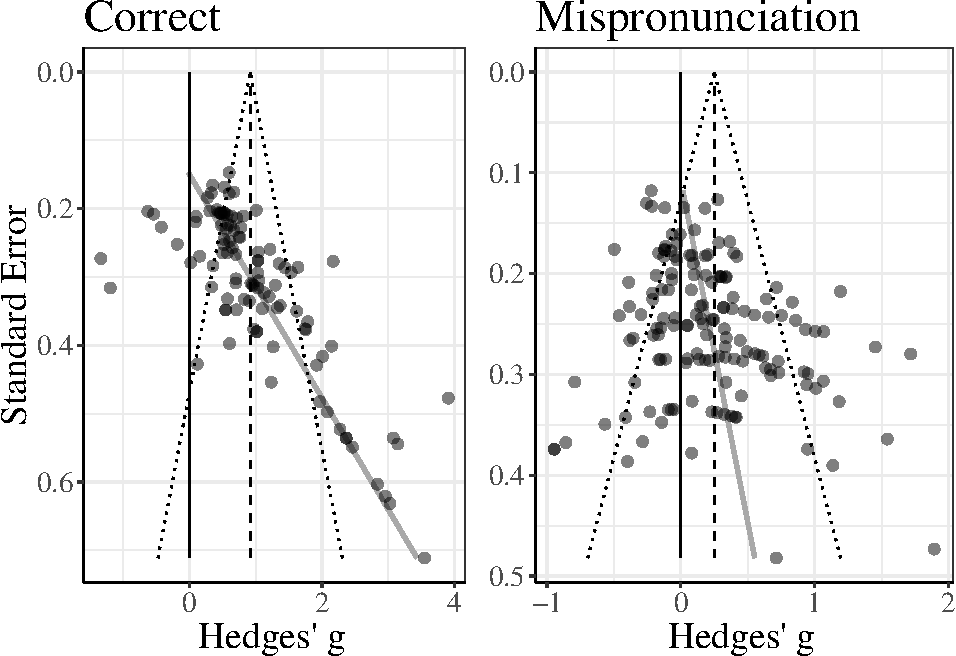
\includegraphics{VonHolzenBergmann_MPMetaAnalysis_files/figure-latex/FunnelCombo-1.pdf}
\caption{\label{fig:FunnelCombo}Funnel plots for object identification,
plotting the standard error of the effect size in relation to the effect
size. The black line marks zero, the dashed grey line marks the effect
estimate, and the grey line marks funnel plot asymmetry.}
\end{figure}

We next examined the p-curves for significant values from the correctly
pronounced and mispronounced conditions. The p-curve based on 72
statistically significant values for correct pronunciations indicates
that the data contain evidential value (Z = -17.93, \emph{p} \textless{}
.001) and we find no evidence of a large proportion of p-values just
below the typical alpha threshold of .05 that researchers consistently
apply in this line of research. The p-curve based on 36 statistically
significant values for mispronunciations indicates that the data contain
evidential value (Z = -6.81, \emph{p} \textless{} .001) and there is
again no evidence of a large proportion of p-values just below the
typical alpha threshold of .05.

Taken together, the results suggest a tendency in the literature towards
publication bias. As a result, our meta-analysis may systematically
overestimate effect sizes and we therefore interpret all estimates with
caution. Yet, the p-curve analysis suggests that the literature contains
evidential value, reflecting a \enquote{real} effect. We therefore
continue our meta-analysis.

\subsection{Meta-analysis}\label{meta-analysis-1}

\subsubsection{Object Identification for Correct and Mispronounced
Words}\label{object-identification-for-correct-and-mispronounced-words}

We first calculated the meta-analytic effect for infants' ability to
identify objects when hearing correctly pronounced labels. The
variance-weighted meta-analytic effect size Hedges' \emph{g} was 0.908
(SE = 0.12) which was significantly different from zero (CI {[}0.673,
1.143{]}, \emph{p} \textless{} .001). This is a small to medium effect
size (according to the criteria set by Mills-Smith, Spangler, Panneton,
\& Fritz, 2015). That the effect size is significantly above zero
suggests that when presented with the correctly pronounced label,
infants tended to fixate on the corresponding object. Although the
publication bias present in our analysis of funnel plot asymmetry
suggests that the effect size Hedges' \emph{g} may be overestimated for
object identification in response to correctly pronounced words, the
p-curve results and a CI lower bound of 0.67, which is substantially
above zero, together suggest that this result is somewhat robust. In
other words, we are confident that the true population mean lies above
zero for object recognition of correctly pronounced words.

We then calculated the meta-analytic effect for object identification in
response to mispronounced words. In this case, the variance-weighted
meta-analytic effect size Hedges' \emph{g} was 0.25 (SE = 0.06) which
was also significantly different from zero (CI {[}0.133, 0.367{]},
\emph{p} \textless{} .001). This is considered a small effect size
(Mills-Smith et al., 2015), but significantly above zero, which suggests
that even when presented with a mispronounced label, infants fixated the
correct object. In other words, infants are able to resolve
mispronunciations, a key skill in language processing We again note the
publication bias (which was smaller in this condition), and the
possibility that the effect size Hedges' \emph{g} may be overestimated.
But, as the p-curve indicated evidential value, we are confident in the
overall pattern, namely that infants fixate the target even after
hearing a mispronounced label.

\subsubsection{Mispronunciation Sensitivity Meta-Analytic
Effect}\label{mispronunciation-sensitivity-meta-analytic-effect}

The above two analyses considered the data from mispronounced and
correctly pronounced words separately. To evaluate mispronunciation
sensitivity, we compared the effect size Hedges' \emph{g} for correct
pronunciations with mispronunciations directly. To this end, we combined
the two datasets. When condition was included (correct, mispronounced),
the moderator test was significant (QM(1) = 215.761, \emph{p}
\textless{} .001). The estimate for mispronunciation sensitivity was
0.495 (SE = 0.034), and infants' looking behavior across conditions was
significantly different (CI {[}0.429, 0.561{]}, \emph{p} \textless{}
.001). This confirms that although infants fixate the correct object for
both correct pronunciations and mispronunciations, the observed
fixations to target (as measured by the effect sizes) were significantly
greater for correct pronunciations. In other words, we observe a
significant difference between the two conditions and can now quantify
the modulation of fixation behavior in terms of standardized effect
sizes and their variance. This first result has both theoretical and
practical implications, as we can now reason about the amount of
perturbation caused by mispronunciations and can plan future studies to
further investigate this effect with suitable power.

Heterogeneity was significant for both correctly pronounced (Q(103) =
625.63, \emph{p} \textless{} .001) and mispronounced words, (Q(146) =
462.51, \emph{p} \textless{} .001), as well as mispronunciation
sensitivity, which included the moderator condition (QE(249) = 1,088.14,
\emph{p} \textless{} .001). This indicated that the sample contains
unexplained variance leading to significant difference between studies
beyond what is to be expected based on random sampling error. We
therefore continue with our moderator analysis to investigate possible
sources of this variance.

\subsubsection{Object Recognition and Mispronunciation Sensitivity
Modulated by
Age}\label{object-recognition-and-mispronunciation-sensitivity-modulated-by-age}

To evaluate the different predictions we laid out in the introduction
for how mispronunciation sensitivity will change as infants develop, we
next added the moderator age (centered; continuous and measured in days
but transformed into months for ease of interpreting estimates by
dividing by 30.44 for Figure \ref{fig:PlotMPEffect}).

In the first analyses, we investigate the impact of age separately on
conditions where words were either pronounced correctly or not. Age did
not significantly modulate object identification in response to
correctly pronounced (QM(1) = 0.678, \emph{p} = 0.41) or mispronounced
words (QM(1) = 1.715, \emph{p} = 0.19). The lack of a significant
modulation together with the small estimates for age (correct: \(\beta\)
= 0.015, SE = 0.018, 95\% CI{[}-0.02, 0.049{]}, \emph{p} = 0.41;
mispronunciation: \(\beta\) = 0.015, SE = 0.011, 95\% CI{[}-0.007,
0.037{]}, \emph{p} = 0.19) indicates that there might be no relationship
between age and target looks in response to a correctly pronounced or
mispronounced label. We note that the estimates in both cases are
positive, however, which is in line with the general assumption that
infants' language processing overall improves as they mature (Fernald et
al., 1998). We plot both object recognition and mispronunciation
sensitivity as a function of age in Figure \ref{fig:PlotMPEffect}.

We then examined the interaction between age and mispronunciation
sensitivity (correct vs.~mispronounced words) in our whole dataset. The
moderator test was significant (QM(3) = 218.621, \emph{p} \textless{}
.001). The interaction between age and mispronunciation sensitivity,
however, was not significant (\(\beta\) = 0.003, SE = 0.008, 95\%
CI{[}-0.012, 0.018{]}, \emph{p} = 0.731); the moderator test was mainly
driven by the difference between conditions. The small estimate, as well
as inspection of Figure \ref{fig:PlotMPEffect}, suggests that as infants
age, their mispronunciation sensitivity neither increases or decreases.

\subsection{(Insert Figure 3 about
here)}\label{insert-figure-3-about-here}

\begin{figure}
\centering
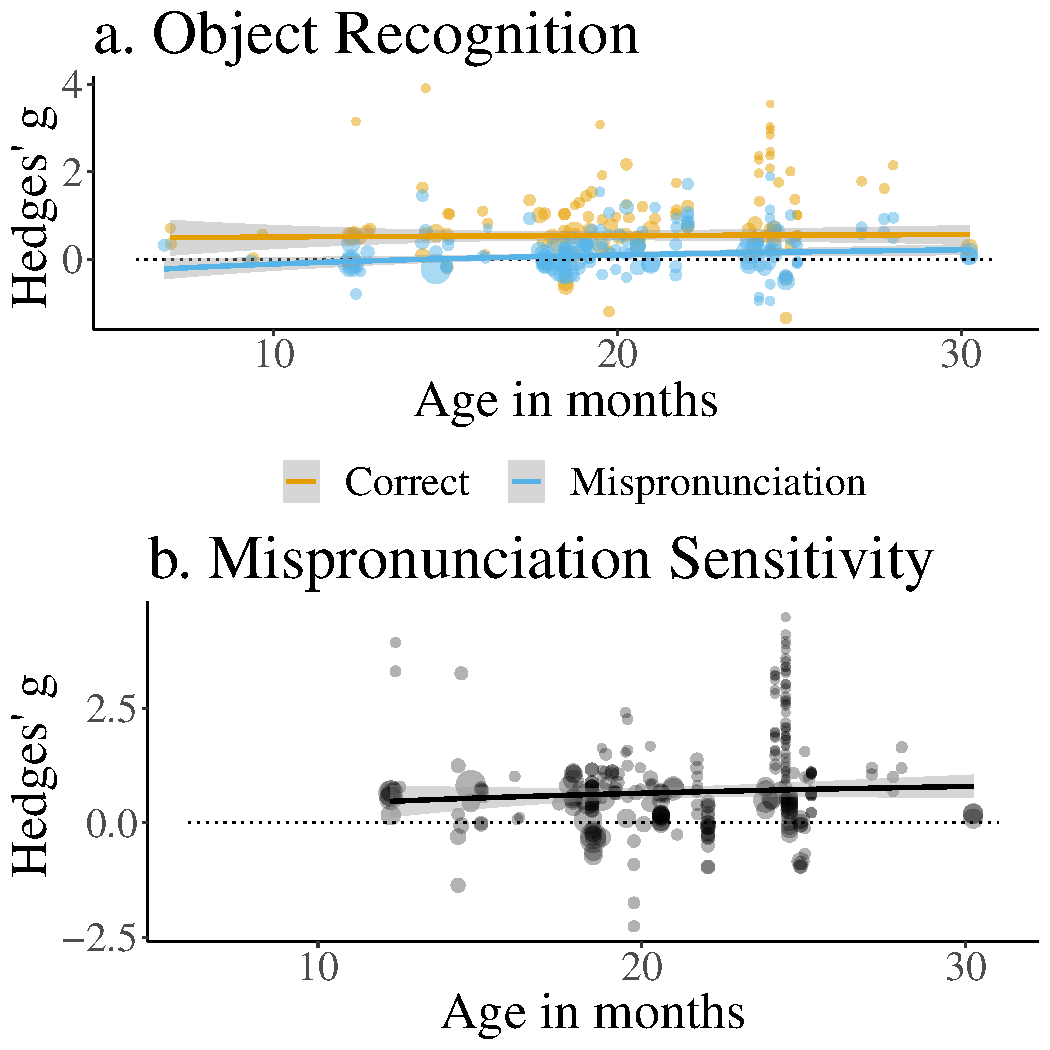
\includegraphics{VonHolzenBergmann_MPMetaAnalysis_files/figure-latex/PlotMPEffect-1.pdf}
\caption{\label{fig:PlotMPEffect}Panel a: Effect sizes for correct
pronunciations (orange) and mispronunciations (blue) by participant age.
Panel b: Effect sizes for mispronunciation sensitivity (correct -
mispronunciations) by participant age. For both panels, point size
depicts inverse variance and the dashed line indicates zero (chance).}
\end{figure}

\subsubsection{Vocabulary Size: Correlation Between Mispronunciation
Sensitivity and
Vocabulary}\label{vocabulary-size-correlation-between-mispronunciation-sensitivity-and-vocabulary}

Of the 32 papers included in the meta-analysis, 13 analyzed the
relationship between vocabulary scores and object recognition for
correct pronunciations and mispronunciations (comprehension = 11 papers
and 39 records; production = 3 papers and 20 records). There is reason
to believe that production data are different from comprehension data.
Children comprehend more words than they can produce, leading to
different estimates for comprehension and production. Production data is
easier to estimate for parents in the typical questionnaire-based
assessment and may therefore be more reliable (Tomasello \& Mervis,
1994). As a result, we planned to analyze these two types of vocabulary
measurement separately. However, because only 3 papers reported
correlations with productive vocabulary scores, only limited conclusions
can be drawn. We also note that because individual effect sizes in our
analysis were related to object recognition and not mispronunciation
sensitivity, we were only able to calculate the relationship between
vocabulary scores and the former. In our vocabulary analysis, we
therefore focus exclusively on the relationship between comprehension
and object recognition for correct pronunciations and mispronunciations.

We first considered the relationship between vocabulary and object
recognition for correct pronunciations. Higher comprehension scores were
associated with greater object recognition in response to correct
pronunciations for 9 of 10 experimental conditions, with correlation
values ranging from -0.16 to 0.48. The weighted mean effect size
Pearson's \emph{r} of 0.14 was small but did differ significantly from
zero (CI {[}0.03; 0.25{]} \emph{p} = 0.012). As a result, we can draw a
tentative conclusion that there is a positive relationship between
comprehension scores and object recognition in response to correct
pronunciations.

We next considered the relationship between vocabulary and object
recognition for mispronunciations. Higher comprehension scores were
associated with greater object recognition in response to
mispronunciations for 17 of 29 experimental conditions, with correlation
values ranging from -0.35 to 0.57. The weighted mean effect size
Pearson's \emph{r} of 0.05 was small and did not differ significantly
from zero (CI {[}-0.01; 0.12{]} \emph{p} = 0.119). The small correlation
suggests either a very small positive or no relationship between
vocabulary and object recognition for mispronunciations. We again
emphasize that we cannot draw a firm conclusion due to the small number
of studies we were able to include here.

Figure \ref{fig:Vocab-describe1} plots the year of publication for all
the mispronunciation sensitivity studies included in this meta-analysis.
This figure illustrates two things: the increasing number of
mispronunciation sensitivity studies and the decreasing number of
mispronunciation studies measuring vocabulary. The lack of evidence for
a relationship between mispronunciation sensitivity and vocabulary size
in some early studies may have contributed to increasingly fewer
researchers including vocabulary measurements in their mispronunciation
sensitivity experimental design. This may explain our underpowered
analysis of the relationship between object recognition for correct
pronunciations and mispronunciations and vocabulary size.

\subsection{(Insert Figure 4 about
here)}\label{insert-figure-4-about-here}

\begin{figure}
\centering
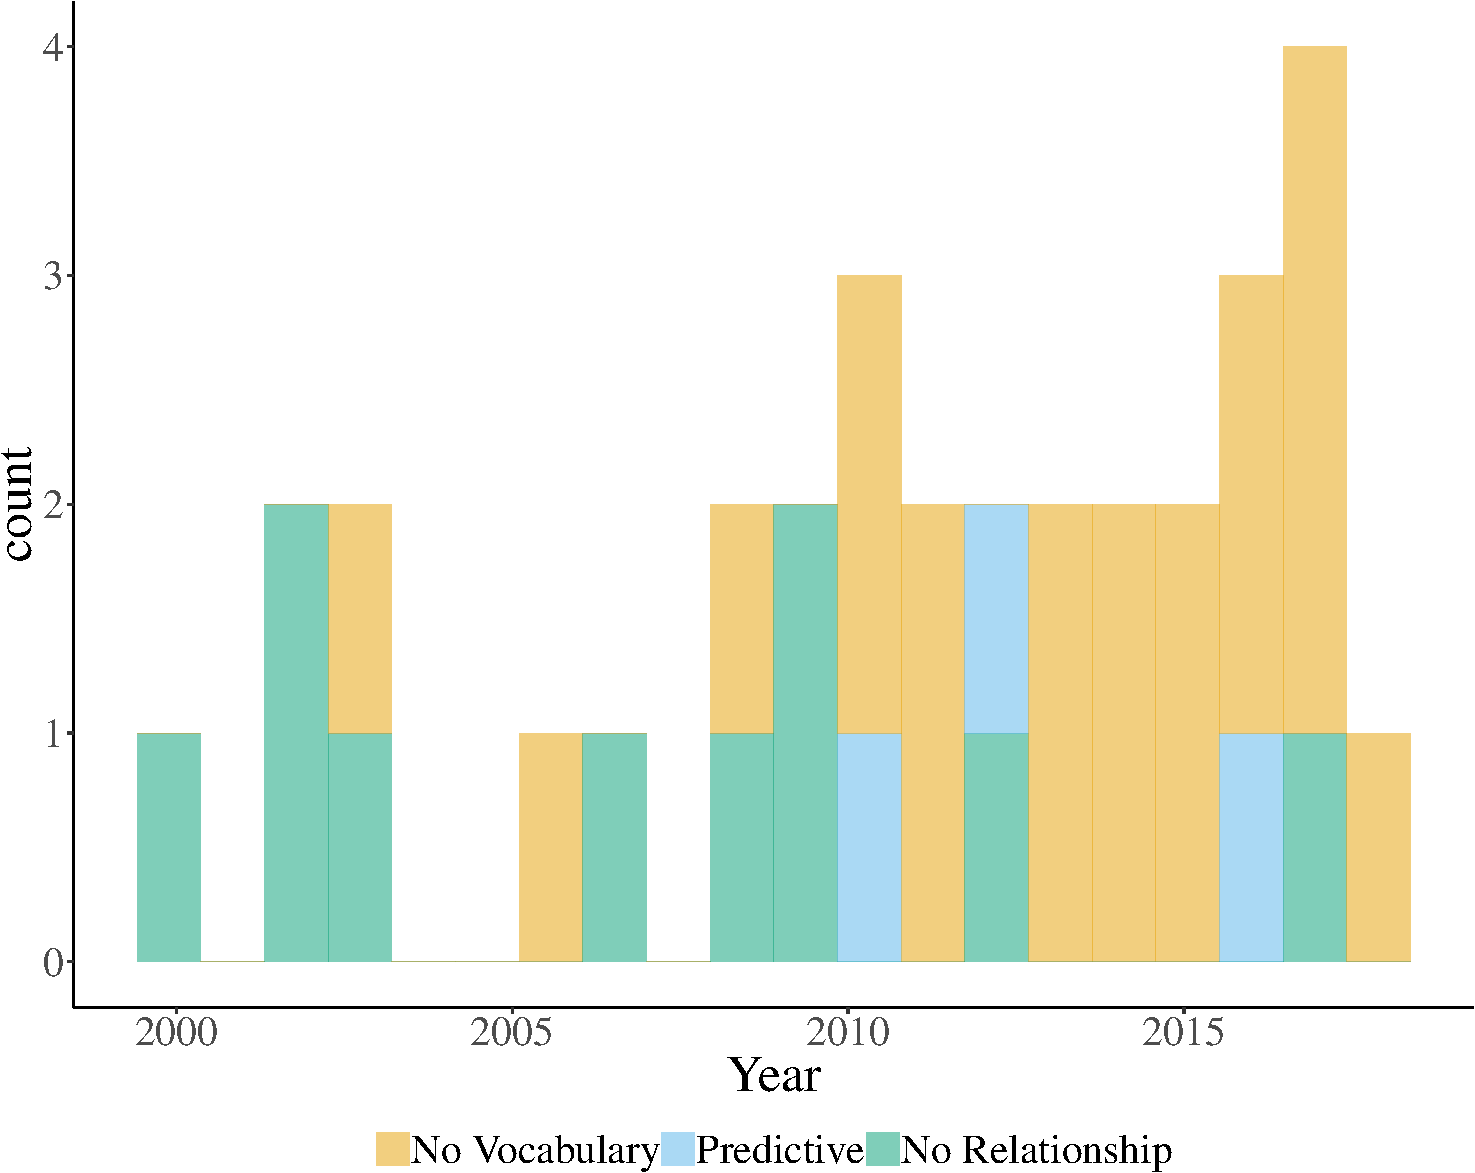
\includegraphics{VonHolzenBergmann_MPMetaAnalysis_files/figure-latex/Vocab-describe1-1.pdf}
\caption{\label{fig:Vocab-describe1}Counts of studies included in the
meta-analysis as a function of publication year, representing whether
the study did not measure vocabulary (orange), did measure vocabulary
and was reported to predict mispronunciation sensitivity (blue), or did
measure vocabulary and was reported to not predict mispronunciation
sensitivity (green).}
\end{figure}

\subsubsection{Interim Discussion}\label{interim-discussion}

The main goal of this paper was to assess mispronunciation sensitivity
and its maturation with age and increased vocabulary size. The results
seem clear: Although infants consider a mispronunciation to be a better
match to the target image than to a distractor image, there was a
constant and stable effect of mispronunciation sensitivity. This did not
change with development, and we might consider age a proxy for
vocabulary size. We observe that the data for directly reported
vocabulary size were too sparse to draw strong conclusions. Of the three
predictions about the development of infants' sensitivity to
mispronunciations discussed in the Introduction, the present results
lend some support for the proposal that mispronunciation sensitivity
stays consistent as infants develop. This runs counter to existing
theories of phono-lexical development, which predict either an increase
(Curtin \& Werker, 2007; Curtin, Byers-Heinlein, \& Werker, 2011; Werker
\& Curtin, 2005) or decrease (Best, 1994, 1995) in mispronunciation
sensitivity. Furthermore, although we found a relationship between
vocabulary size (comprehension) and target looking for correct
pronunciations, we found no relationship between vocabulary and target
looking for mispronunciations. This also runs counter to the predictions
for the PRIMR (Curtin \& Werker, 2007; Curtin et al., 2011; Werker \&
Curtin, 2005) and Assimilation (Best, 1994, 1995) models, but may be due
to our analyses being underpowered. In sum, it seems that current
theories of infants' phono-lexical development cannot fully capture our
results, but that more investigation is needed to draw a firm
conclusion.

Alternatively, an effect of maturation might have been masked by other
factors we have not yet captured in our analyses. A strong candidate
that emerged during the construction of the present dataset and careful
reading of the original papers was the analysis approach. We observed,
as mentioned in the Methods section, large variation in the dependent
variable reported, and additionally noted that the size of the chosen
post-naming analysis window varied substantially across papers.
Researchers might adapt their analysis strategy to infants' age or they
might be influenced by having observed the data. For example, consider
the possibility that there is a true increase in mispronunciation
sensitivity over development. In this scenario, younger infants should
show no or only little sensitivity to mispronunciations while older
infants would show a large sensitivity to mispronunciations. This lack
of or small mispronunciation sensitivity in younger infants is likely to
lead to non-significant results, which would be more difficult to
publish (C. J. Ferguson \& Heene, 2012). In order to have publishable
results, adjustments to the analysis approach could be made until a
significant, but spurious, effect of mispronunciation sensitivity is
found. This would lead to an increase in significant results and alter
the observed developmental trajectory of mispronunciation sensitivity.
Such a scenario is in line with the publication bias we observe
(Simmons, Nelson, \& Simonsohn, 2011). We examine whether variation in
the approach to data analysis may be have an influence on our
conclusions regarding infants' developing mispronunciation sensitivity.

We included details related to timing and type of dependent variable in
our coding of the dataset because they are consistently reported and
might be useful for experiment design in the future by highlighting
typical choices and helping establish field standards. In the following
section, we include an exploratory analysis to investigate the
possibility of systematic differences in the approach to analysis in
general and across infant age. The purpose of this analysis was to
better understand the influence of choices made in analyzing
mispronunciation sensitivity studies as well as the influence these
choices may have on our understanding of mispronunciation sensitivity
development.

\subsection{Exploratory Analyses}\label{exploratory-analyses}

We identified two sets of variables which varied across papers to assess
the influence of data analysis choices on resulting effect size: timing
(post-naming analysis window; offset time) and which dependent
variable(s) were reported. In the following, we discuss the possible
theoretical motivation for these data analysis choices, the variation
present in the current meta-analysis dataset, and the influence these
analysis choices may have on measurements of mispronunciation
sensitivity development. We focus specifically on the size of the
mispronunciation sensitivity effect, considering the whole dataset and
including condition (correct pronunciation, mispronunciation) as
moderator.

\subsubsection{Timing}\label{timing}

In a typical trial in a mispronunciation sensitivity study, the
target-distractor image pairs are first presented in silence, followed
by auditory presentation of a carrier phrase or isolated presentation of
the target word (correctly pronounced or mispronounced). When designing
mispronunciation sensitivity studies, experimenters can choose the
length of time each trial is presented. This includes both the length of
time before the target object is named (pre-naming phase) as well as
after (post-naming phase) and is determined prior to data collection. To
examine the size of the time window analyzed in the post-naming phase
(post-naming analysis window), we must first consider overall length of
time in post-naming (post-naming time window), because it limits the
overall time window available to analyze and might thus predict the
post-naming analysis window. Across papers, the length of the
post-naming time window varied from 2000 to 9000 ms, with a median value
of 3500 ms. The most popular post-naming time window length was 4000 ms,
used in 74 experimental conditions. There was no apparent relation
between infant age and post-naming time window length (\emph{r} = 0.01,
95\% CI{[}-0.11, 0.13{]}, \emph{p} = 0.882).

Unlike the post-naming time window, the post-naming analysis window can
be chosen after the experimental data is collected. Interestingly, half
of the experimental conditions were analyzed using the whole post-naming
time window of the trial presented to the infant (\emph{n} = 124), while
the other half were analyzed using a shorter portion of the post-naming
time window, usually excluding later portions (\emph{n} = 127). Across
papers, the length of the post-naming analysis window varied from 1510
to 4000 ms, with a median value of 2500 ms. The most popular post-naming
analysis window length was 2000 ms, used in 97 experimental conditions.
There was an inverse relationship between infant age and post-naming
analysis window length, such that younger infants' looking times were
analyzed using a longer post-naming analysis window, here the
relationship was significant (\emph{r} = -0.23, 95\% CI{[}-0.35,
-0.11{]}, \emph{p} \textless{} .001). The choice to use a shorter
post-naming analysis window with age is likely related to evidence that
speed of processing is slower in younger infants (Fernald et al., 1998).
To summarize, we observe variation in time-related analysis decisions
related to infants' age.

Another potential source of variation in studies that analyze
eye-movements is the amount of time it takes for an eye movement to be
initiated in response to a visual stimulus, which we refer to as offset
time. Previous studies examining simple stimulus response latencies
first determined that infants require at least 233 ms to initiate an
eye-movement in response to a stimulus (Canfield \& Haith, 1991). In the
first infant mispronunciation sensitivity study, Swingley and Aslin
(2000) used an offset time of 367 ms, which was \enquote{an
\enquote{educated guess} based on studies . . . showing that target and
distractor fixations tend to diverge at around 400 ms.} (Swingley \&
Aslin, 2000, p. 155). Upon inspecting the offset time values used in the
papers in our meta-analysis, the majority used a similar offset time
value (between 360 and 370 ms) for analysis (\emph{n} = 151), but offset
values ranged from 0 to 500 ms, and were not reported for 36
experimental conditions. We note that Swingley (2009) also included
offset values of 1133 ms to analyze responses to coda mispronunciations.
There was an inverse relationship between infant age and size of offset,
such that younger infants were given longer offsets, although this
correlation was not significant (\emph{r} = -0.10, 95\% CI{[}-0.23,
0.03{]}, \emph{p} = 0.13). This lack of a relationship is possibly
driven by the field's consensus that an offset of about 367 ms is
appropriate for analyzing word recognition with PTL measures, including
studies that evaluate mispronunciation sensitivity.

Although there are a priori reasons to choose the post-naming analysis
window (infant age) or offset time (previous studies), these choices may
occur after data collection and might therefore lead to a higher rate of
false-positives (Gelman \& Loken, 2013). Considering that these choices
were systematically different across infant ages, at least for the
post-naming analysis window, we next explored whether the post-naming
analysis window length or the offset time influenced our estimate of
infants' sensitivity to mispronunciations.

\paragraph{Post-naming analysis window
length}\label{post-naming-analysis-window-length}

We first assessed whether size of the post-naming analysis window had an
impact on the overall size of the reported mispronunciation sensitivity.
We considered data from both conditions in a joint analysis and included
condition (correct pronunciation, mispronunciation) as an additional
moderator. The moderator test was significant (QM(3) = 236.958, \emph{p}
\textless{} .001). The estimate for the interaction between post-naming
analysis window and condition was small but significant (\(\beta\) =
-0.262, SE = 0.059, 95\% CI{[}-0.377, -0.148{]}, \emph{p} \textless{}
.001). This relationship is plotted in Figure
\ref{fig:Plot-post-name-cond-age}a. The results suggest that the size of
the post-naming analysis window significantly impacted our estimate of
mispronunciation sensitivity. Specifically, the difference between
target fixations for correctly pronounced and mispronounced items
(mispronunciation sensitivity) was significantly greater when the
post-naming analysis window was shorter.

Considering that we found a significant relationship between the length
of the post-naming analysis window and infant age, such that younger
ages had a longer window of analysis, we next examined whether the size
of the post-naming analysis window modulated the estimated size of
mispronunciation sensitivity as infant age changed. We therefore
included age as additional moderator of the previous analysis. The
moderator test was significant (QM(7) = 247.322, \emph{p} \textless{}
.001). The estimate for the three-way-interaction between condition,
size of the post-naming analysis window, and age was small, but
significant (\(\beta\) = -0.04, SE = 0.014, 95\% CI{[}-0.068, -0.012{]},
\emph{p} = 0.006). As can be seen in Figure
\ref{fig:Plot-post-name-cond-age}b, a smaller post-naming analysis
window leads to a greater increase in measured mispronunciation
sensitivity with development. For example, when experimental conditions
were analyzed with a post-naming analysis window of 2000 ms or less,
mispronunciation sensitivity seems to increase with infant age. If the
post-naming analysis window is greater than 2000 ms, however, there is
no or a negative relation of mispronunciation sensitivity and age. In
other words, all three possible developmental hypotheses might be
supported depending on analysis choices made regarding the size of the
post-naming analysis window. This is especially important, considering
that our key question is how mispronunciation sensitivity changes with
development. These results suggest that conclusions about the
relationship between infant age and mispronunciation sensitivity may be
mediated by the size of the post-naming analysis window.

\subsection{(Insert Figure 5 about
here)}\label{insert-figure-5-about-here}

\begin{figure}
\centering
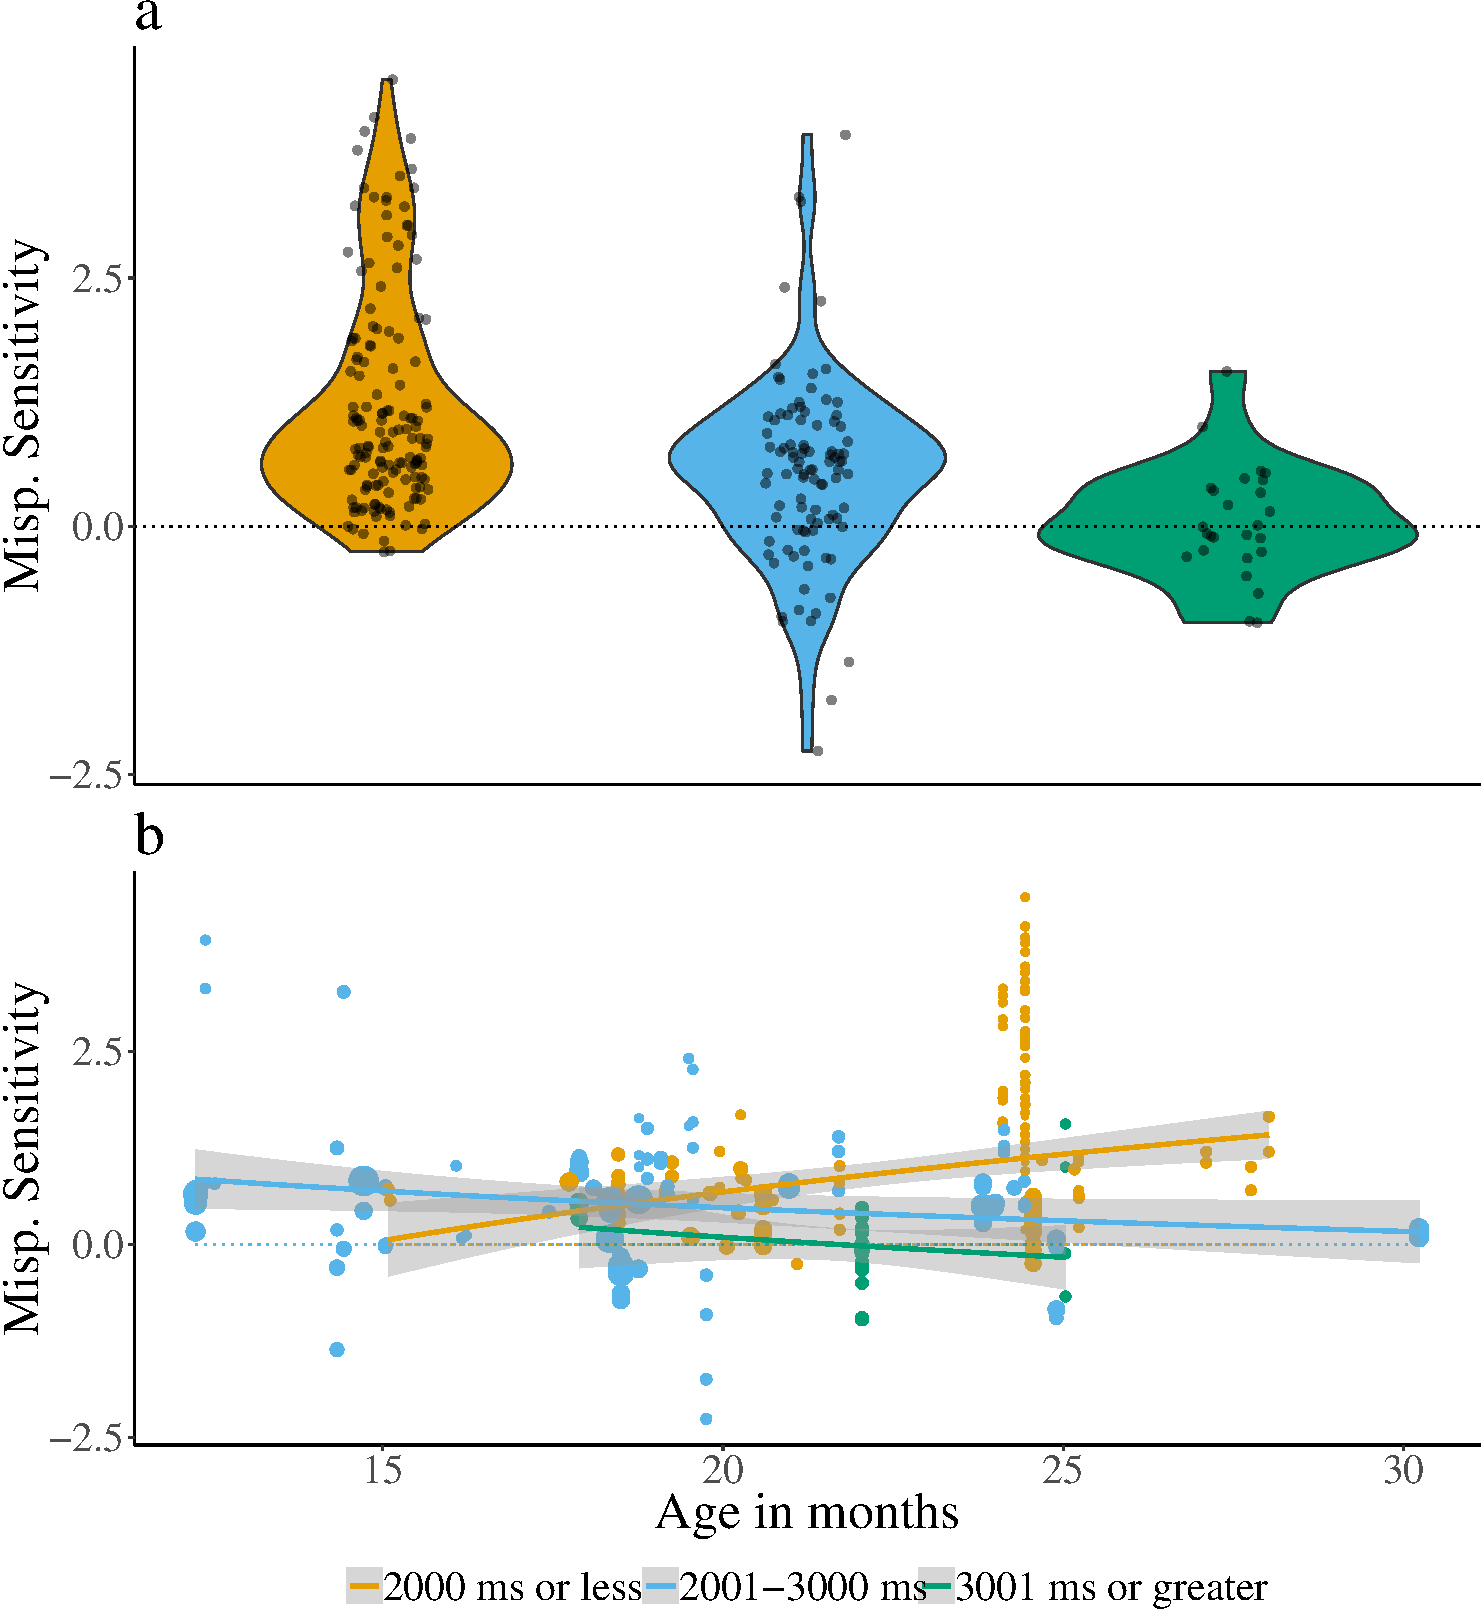
\includegraphics{VonHolzenBergmann_MPMetaAnalysis_files/figure-latex/Plot-post-name-cond-age-1.pdf}
\caption{\label{fig:Plot-post-name-cond-age}Effect sizes for the different
lengths of the post-naming analysis window: 2000 ms or less (orange),
2001 to 3000 ms (blue), and 3001 ms or greater (green). Although length
of the post-naming analysis window was included as a continuous variable
in the meta-analytic model, it is divided into categories for ease of
viewing. Panel a plots mispronunciation sensitivity aggregated over age,
while panel b plots mispronunciation sensitivity as a function of age.
The lines plot the linear regression and the gray shaded area indicates
the standard error.}
\end{figure}

\paragraph{Onset time after target
naming}\label{onset-time-after-target-naming}

We next assessed whether the time between target naming and the start of
the analysis, namely offset time, had an impact on the size of the
reported mispronunciation sensitivity. When we included both condition
and offset time as moderators, the moderator test was significant (QM(3)
= 236.958, \emph{p} \textless{} .001), but the estimate for the
interaction between offset time and condition was zero (\(\beta\) = 0,
SE = 0, 95\% CI{[}-0.001, 0{]}, \emph{p} = 0.505). Although we found no
relationship between offset time and infant age, we also examined
whether the size of offset time modulated the measure of
mispronunciation sensitivity over infant age. When both offset time and
condition were included as moderators, the moderator test was
significant (QM(7) = 200.867, \emph{p} \textless{} .001), but the
three-way-interaction between condition, offset time, and age was again
zero (\(\beta\) = 0, SE = 0, 95\% CI{[}0, 0{]}, \emph{p} = 0.605). Taken
together, these results suggest that offset time does not modulate
measured mispronunciation sensitivity. There is no relationship between
offset time and age, and we find no influence of offset time on the
estimated size of mispronunciation sensitivity over age. We again point
out that there is a substantial field consensus, which might mask any
relationship.

\subsubsection{Dependent variable-related
analyses}\label{dependent-variable-related-analyses}

Mispronunciation studies evaluate infants' proportion of target looks
(PTL) in response to correct and mispronounced words. Experiments
typically include a phase where a naming event has not yet occurred,
which we refer to as the pre-naming phase. This is followed by a naming
event, whether correctly pronounced or mispronounced, and the subsequent
phase we refer to as the post-naming phase. The purpose of the
pre-naming phase is to ensure that infants do not have systematic
preferences for the target or distractor (greater interest in a cat
compared to a cup) which may drive PTL scores in the post-naming phase.
As described in the Data Analysis sub-section of the Methods, however,
there was considerable variation across papers in whether this
pre-naming phase was used as a baseline measurement, or whether a
different baseline measurement was used. This resulted in different
measured outcomes or dependent variables. Over half of the experimental
conditions (\emph{n} = 129) subtracted the PTL score for a pre-naming
phase from the PTL score for a post-naming phase, resulting in a
Difference Score. The Difference Score is one value, which is then
compared with a chance value of 0. When positive, this indicates that
infants increased their looks to the target after hearing the naming
label (correct or mispronounced) relative to the pre-naming baseline
PTL. In contrast, Pre vs.~Post (\emph{n} = 69 experimental conditions),
directly compare the post- and pre-naming PTL scores with one another
using a statistical test (e.g.~t-test, ANOVA). This requires two values,
one for the pre-naming phase and one for the post-naming phase. A
greater post compared to pre-naming phase PTL indicates that infants
increased their target looks after hearing the naming label. The
remaining experimental conditions used a Post dependent variable
(\emph{n} = 53 experimental conditions), which compares the post-naming
PTL score with a chance value of 50\%. Here, the infants' pre-naming
phase baseline preferences are not considered and instead target
fixations are evaluated based on the likelihood to fixate one of two
pictures (50\%). As most papers do not specify whether these
calculations are made before or after aggregating across trials, we make
no assumptions about when this step is taken.

The Difference Score and Pre vs.~Post can be considered similar to one
another, in that they are calculated on the same type of data and
consider pre-naming preferences. It should be noted, however, that the
Difference Score may better counteract participant- and item-level
differences, whereas Pre vs.~Post is a group-level measure. The Post
dependent variable, in contrast, does not consider pre-naming baseline
preferences. To our knowledge, there is no theory or evidence that
explicitly drives choice of dependent variable in analysis of
mispronunciation sensitivity, which may explain the wide variation in
dependent variable reported in the papers included in this
meta-analysis. We next explored whether the type of dependent variable
calculated influenced the estimated size of sensitivity to
mispronunciations. Considering that the dependent variable Post differs
in its consideration of pre-naming baseline preferences, substituting
these for a chance value, we directly compared mispronunciation
sensitivity between Post as a reference condition and both Difference
Score and Pre vs.~Post dependent variables.

We first assessed whether the choice of dependent variable had an impact
on the size of estimated mispronunciation sensitivity. When we included
both condition and dependent variable as moderators, the moderator test
was significant (QM(5) = 259.817, \emph{p} \textless{} .001). The
estimate for the interaction between Pre vs.~Post and condition was
significantly smaller than that of the Post dependent variable
(\(\beta\) = -0.392, SE = 0.101, 95\% CI{[}-0.59, -0.194{]}, \emph{p}
\textless{} .001), but the difference between the Difference Score and
Post in the interaction with condition was small and not significant
(\(\beta\) = -0.01, SE = 0.098, 95\% CI{[}-0.203, 0.183{]}, \emph{p} =
0.916). This relationship is plotted in Figure
\ref{fig:Plot-Within-cond-age-diff-score}a. The results suggest that the
reported dependent variable significantly impacted the size of the
estimated mispronunciation sensitivity effect, such that studies
reporting the Post. vs.~Pre dependent variable showed a smaller
mispronunciation sensitivity effect than those reporting Post, but that
there was no difference between the Difference Score and Post dependent
variables.

We next examined whether the type of dependent variable calculated
modulated the estimated change in mispronunciation sensitivity over
infant age. When age was included as an additional moderator, the
moderator test was significant (QM(11) = 273.585, \emph{p} \textless{}
.001). The estimate for the interaction between Pre vs.~Post, condition,
and age was significantly smaller than that of the Post dependent
variable (\(\beta\) = -0.089, SE = 0.03, 95\% CI{[}-0.148, -0.03{]},
\emph{p} = 0.003), but the difference between the Difference Score and
Post in the interaction with condition and age was small and not
significant (\(\beta\) = -0.036, SE = 0.027, 95\% CI{[}-0.088, 0.016{]},
\emph{p} = 0.174). This relationship is plotted in Figure
\ref{fig:Plot-Within-cond-age-diff-score}b. When the dependent variable
reported was Pre vs.~Post, mispronunciation sensitivity was found to
decrease with infant age, while in comparison, when the dependent
variable was Post, mispronunciation sensitivity was found to increase
with infant age. There was no difference in the estimated
mispronunciation sensitivity change with infant age between the Post and
Difference Score dependent variables.

Similar to the length of the post-naming analysis window, all three
possible developmental hypotheses might be supported depending on the
dependent variable reported. In other words, choice of dependent
variable may influence the conclusion drawn regarding how
mispronunciation sensitivity may change with infant age.

\subsection{(Insert Figure 6 about
here)}\label{insert-figure-6-about-here}

\begin{figure}
\centering
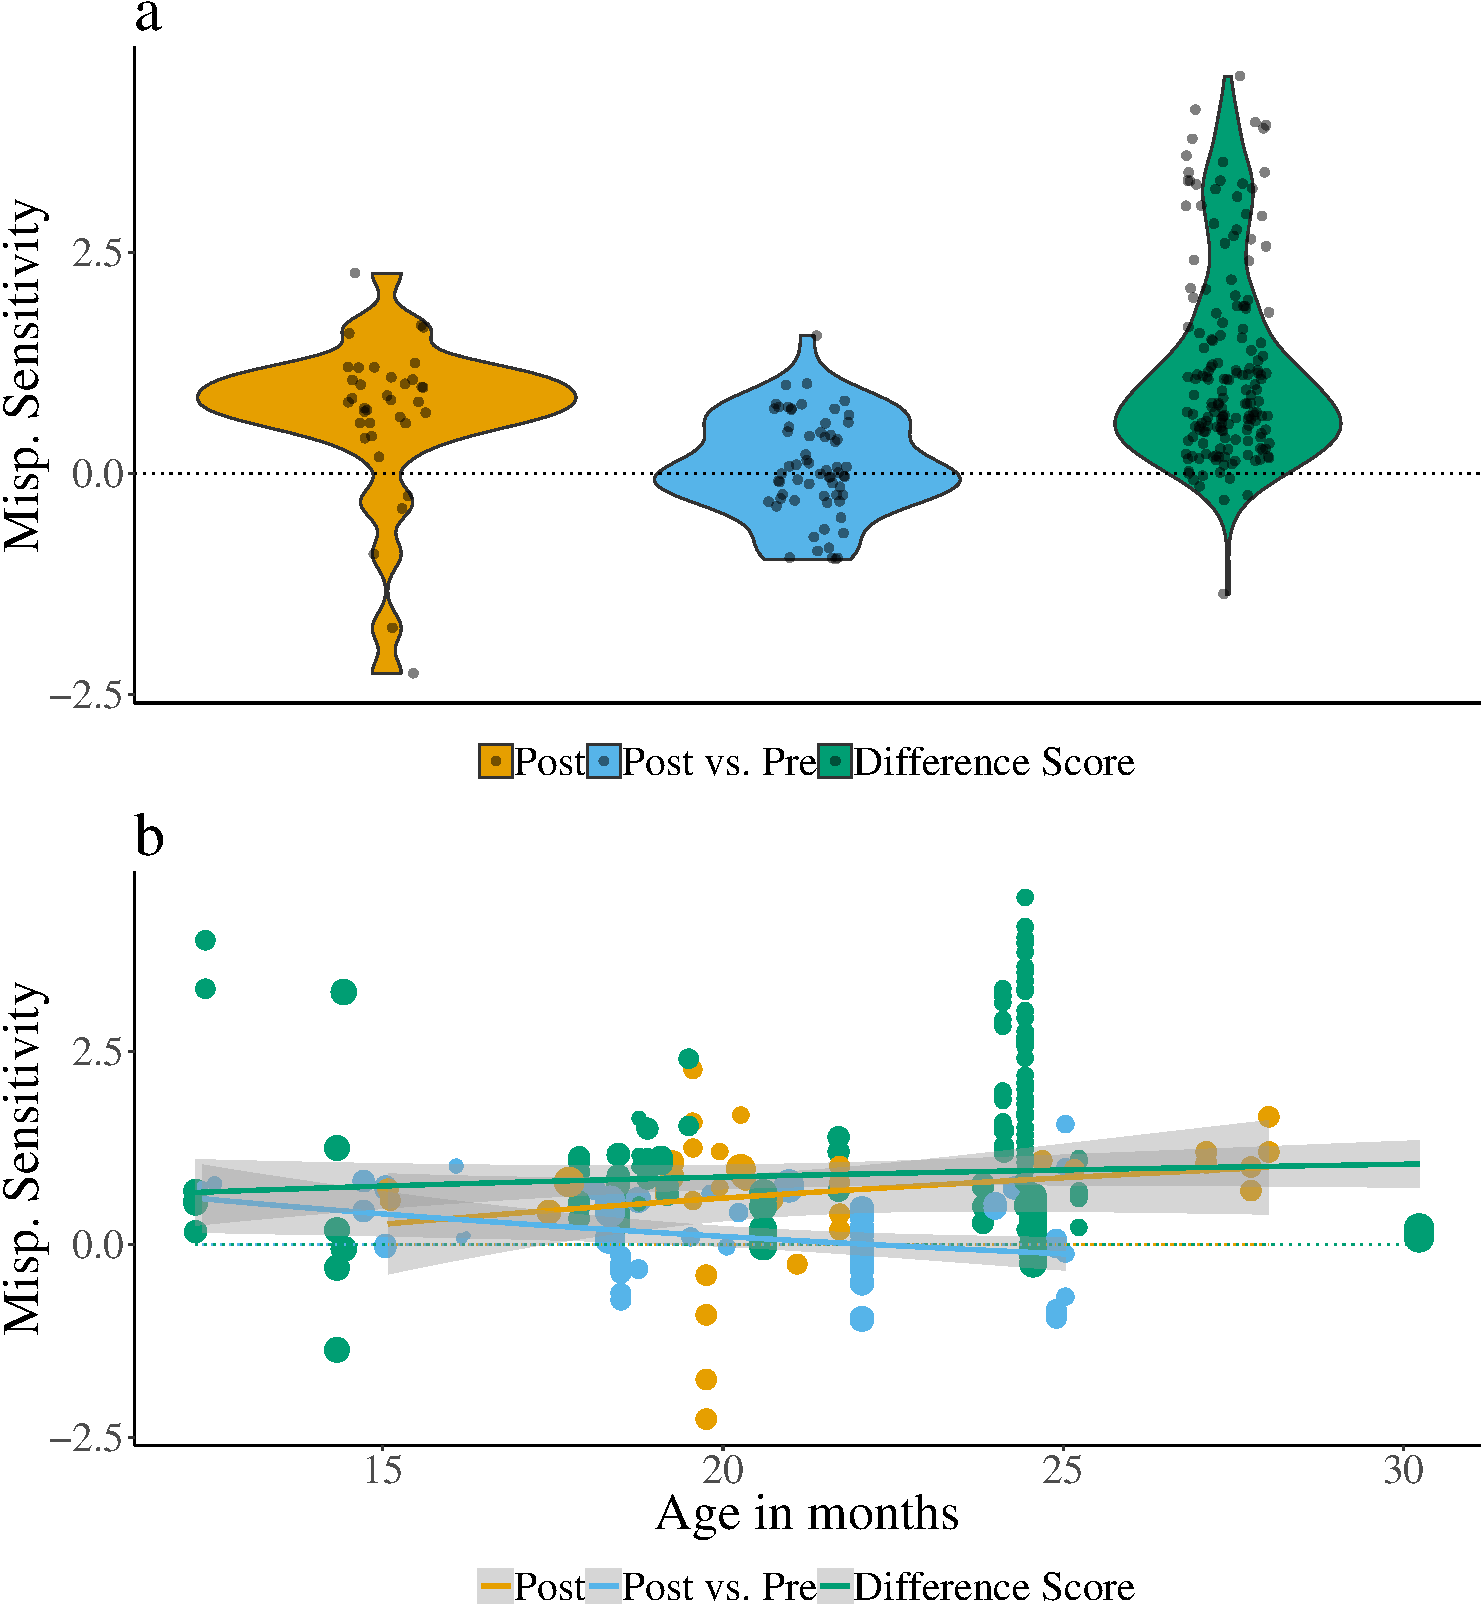
\includegraphics{VonHolzenBergmann_MPMetaAnalysis_files/figure-latex/Plot-Within-cond-age-diff-score-1.pdf}
\caption{\label{fig:Plot-Within-cond-age-diff-score}Effect sizes for the
different types of dependent variables calculated: Post (orange), Post
vs.~Pre (blue), and Difference Score (green). Panel a plots
mispronunciation sensitivity aggregated over age, while panel b plots
mispronunciation sensitivity as a function of age. The lines plot the
linear regression and the gray shaded area indicates the standard
error.}
\end{figure}

\section{General Discussion}\label{general-discussion}

In this meta-analysis, we set out to quantify and assess the
developmental trajectory of infants' sensitivity to mispronunciations.
Overall, the results of the meta-analysis showed that infants reliably
fixate the target object when hearing both correctly pronounced and
mispronounced labels. Infants not only recognize object labels when they
were correctly pronounced, but are also likely to accept
mispronunciations as labels for targets, in the presence of a distractor
image. Nonetheless, there was a considerable difference in target
fixations in response to correctly pronounced and mispronounced labels,
suggesting that infants show an overall mispronunciation sensitivity
based on the current experimental literature. In other words, infants
show sensitivity to what constitutes unacceptable, possibly
meaning-altering variation in word forms, thereby displaying knowledge
of the role of phonemic changes throughout the ages assessed here (6 to
30 months). At the same time, infants, like adults, can recover from
mispronunciations, a key skill in language processing.

We next evaluated the developmental trajectory of infants'
mispronunciation sensitivity. Based on previous theoretical accounts and
existing experimental evidence, we envisioned three possible
developmental patterns: increasing, decreasing, and unchanging
sensitivity. We observed no influence of age when it was considered as a
moderator of mispronunciation sensitivity. Of the two mainstream
theories identified in our literature review, neither the Perceptual
Attunement account (Best, 1994, 1995) nor PRIMIR (Curtin \& Werker,
2007; Curtin et al., 2011; Werker \& Curtin, 2005) account for a lack of
developmental change. The results of our meta-analysis are reflecting a
pattern previously reported by a handful of studies directly comparing
infants over a range of ages (Bailey \& Plunkett, 2002; Swingley \&
Aslin, 2000; Zesiger et al., 2012), which also found no developmental
change in mispronunciation sensitivity.

Both the Perceptual Attunement (Best, 1994, 1995) and PRIMIR (Curtin \&
Werker, 2007; Curtin et al., 2011; Werker \& Curtin, 2005) accounts link
a change of mispronunciation sensitivity specifically with vocabulary
growth, in comparison to development in general. Vocabulary growth is
predicted to lead either to an increase (PRIMIR; Curtin \& Werker, 2007;
Curtin et al., 2011; Werker \& Curtin, 2005) or a decrease (Perceptual
Attunement; Best, 1994, 1995) in mispronunciation sensitivity;
vocabulary has been shown to grow considerably in the age range
considered in the current meta-analysis (see
\url{http://wordbank.stanford.edu}; Frank et al., 2017). However, there
are also substantial individual differences in the trajectory of
vocabulary growth. The lack of developmental effects found in our
meta-analysis may therefore be due to using age, instead of vocabulary
size, as a moderator of mispronunciation sensitivity. We tried to
address this issue by conducting an analysis of the subset of studies
reporting correlations between infants' vocabulary size and their
responses to correct and mispronounced labels. However, this analysis
relied on only a few papers. We observed that an increasing vocabulary
size lead to increased object recognition for correctly pronounced
words; this was not the case for mispronunciations. However, it is
difficult to draw any strong conclusions regarding the role of an
increasing vocabulary size in mispronunciation sensitivity from this
data.

Why did we have so few samples for an analysis on vocabulary size to
begin with? Despite the theoretical implications, fewer than half of the
papers included in this meta-analysis measured vocabulary (\emph{n} =
13; out of 32 papers total; see also Figure \ref{fig:Vocab-describe1}).
There are more mispronunciation sensitivity studies published every
year, perhaps due to the increased use of eye-trackers, which reduce the
need for offline coding and thus make data collection much more
efficient, but this has not translated to an increasing number of
mispronunciation sensitivity studies also reporting vocabulary scores.
We suggest that this may be the result of publication bias favoring
significant effects or an overall hesitation to invest in data
collection that is not expected to yield significant outcomes.

What do our (tentative) results mean for theories of language
development? Evidence that infants accept a mispronunciation (object
identification) while simultaneously holding correctly pronounced and
mispronounced labels as separate (mispronunciation sensitivity) may
indicate an abstract understanding of words' phonological structure
being in place early on. It appears that young infants may understand
that the phonological form of mispronunciations and correct
pronunciations do not match (phonological distinctiveness), but that the
mispronunciation is a better label for the target compared to the
distractor image (phonological constancy). The lack of age or vocabulary
effects in our meta-analysis suggest that this understanding is present
from an age when the earliest words are learned and is maintained
throughout early lexical development. This implies mastery of the
principles of phonological constancy and phonological distinctiveness at
an age earlier than previously thought, which we recommend should be
further explored experimentally and taken into consideration by future
theoretical accounts.

\subsection{Data Analysis Choices}\label{data-analysis-choices}

While creating the dataset on which this meta-analysis was based, we
included as many details as possible to describe each study. During the
coding of these characteristics, we noted a potential for variation in a
handful of variables that relate to data analysis, specifically relating
to timing (post-naming analysis window; onset time) and to the
calculation of the dependent variable reported. We focused on these
variables in particular because their choice can potentially be made
after researchers have examined the data, leading to an inflated number
of significant results which may also explain the publication bias
observed in the funnel plot asymmetry analyses (Simmons et al., 2011).
To explore whether this variation contributed to the lack of
developmental change observed in the overall meta-analysis, we included
these variables as moderators in a set of exploratory analyses. We noted
an interesting pattern of results, specifically that different
conclusions about mispronunciation sensitivity, but more notably
mispronunciation sensitivity development, could be drawn depending on
the length of the post-naming analysis window as well as the type of
dependent variable calculated in the experiment (see Figures
\ref{fig:Plot-post-name-cond-age} and
\ref{fig:Plot-Within-cond-age-diff-score}).

Infants recognize words more quickly with age (Fernald et al., 1998),
which has the potential to influence decisions for the analysis of the
post-naming time window in mispronunciation sensitivity studies,
including where to begin the time window (onset time) and how long this
analysis window should be (post-naming analysis window). For example, as
age increases, reaction time should increase and experimenters may
adjust and lower offset times in their analysis as well as shorten the
length of the analysis window. Yet, we find no relationship between age
and offset times, nor that offset time modulated mispronunciation
sensitivity. Indeed, a majority of studies used an offset time between
360 and 370 ms, which follows the \enquote{best guess} of Swingley and
Aslin (2000) for the amount of time needed for infants to initiate eye
movements in response to a spoken target word. Without knowledge of the
base reaction time in a given population of infants, use of this best
guess offset time reduces the number of free parameters. In contrast, we
found a negative correlation between infant age and the length of the
post-naming analysis window, and that the length of the analysis window
moderated mispronunciation sensitivity, such increasing the length of
the analysis windows decreases the size of mispronunciation sensitivity.
Given a set of mispronunciation sensitivity data, a conclusion regarding
the development of mispronunciation sensitivity would be different
depending on the length of the post-naming analysis window. Although we
have no direct evidence, an analysis window can be potentially set after
collecting data. At worst, this adjustment could be the result of a
desire to confirm a hypothesis, increasing the rate of false-positives
(Gelman \& Loken, 2013): a \enquote{significant effect} of
mispronunciation sensitivity is found with an analysis window of 2000
but not 3000 ms, therefore 2000 ms is chosen. At best, this variation
introduces noise into the study of mispronunciation sensitivity, bluring
the true developmental trajectory of mispronunciation sensitivity. In
the next section, we highlight some suggestions for how the field can
remedy this issue.

Surpisingly, we found that the type of dependent variable calculated
moderated mispronunciation sensitivity and conclusions about its
developmental trajectory. Unlike the exploratory analyses related to
timing (onset and post-naming analysis window), there is not a clear
reason for one dependent variable to be chosen over another; the
prevelence of each dependent variable appears distributed across ages
and some authors always calculate the same dependent variable while
others use them interchangeably in different publications. One clear
difference is that both the Difference Score and Pre vs.~Post dependent
variables take into account each infants' actual preference in the
pre-naming baseline phase, while the Post dependent variable does not.
Without access to the raw data, it is difficult to conclusively
determine why different dependent variable calculations influence
mispronunciation sensitivity. In the next section, we advocate for the
adoption of Open Data practices as one way to address this issue.

\subsection{Recommendations to Establish Analysis
Standards}\label{recommendations-to-establish-analysis-standards}

A lack of a field standard can have serious consequences, as our
analyses show. Depending on which analysis time window (see Figure
\ref{fig:Plot-post-name-cond-age}) or dependent variable (see Figure
\ref{fig:Plot-Within-cond-age-diff-score}) we focus on, we find support
for any of the three possible trajectories of mispronunciation
sensitivity development. On the one hand, this limits the conclusions we
can draw regarding our key research question. Without access to the full
datasets or analysis code of the studies included in this meta-analysis,
it is difficult to pinpoint the exact role played by these data analysis
choices. On the other hand, this finding emphasizes that current
practices of free, potentially ad hoc choices regarding data analyses
are not sustainable if the field wants to move towards quantitative
evidence for theories of language development.

We take this opportunity to suggest several recommendations to address
the issue of potential posthoc analysis decisions. Preregistration can
serve as proof of a priori decisions regarding data analysis, which can
also contain a data-dependent description of how data analysis decisions
will be made once data is collected. The peer-reviewed form of
preregistration, termed Registered Reports, has already been adopted by
a large number of developmental journals, and general journals that
publish developmental works, showing the field's increasing acceptance
of such practices for hypothesis-testing studies. Sharing data (Open
Data) can allow others to re-analyze existing datasets to both examine
the impact of analysis decisions and cumulatively analyze different
datasets in the same way. Considering the issue of analysis time window,
experimenters can opt to analyze the time course as a whole, instead of
aggregating the proportion of target looking behavior over the entire
trial. This allows for a more detailed assessment of infants' fixations
over time and reduces the need to reduce the post-naming analysis
window. Both Growth Curve Analysis (Law II \& Edwards, 2015; Mirman,
Dixon, \& Magnuson, 2008) and Permutation Clusters Analysis (Delle
Luche, Durrant, Poltrock, \& Floccia, 2015; Maris \& Oostenveld, 2007;
Von Holzen \& Mani, 2012) offer potential solutions to analyze the full
time course. Furthermore, it may be useful to establish standard
analysis pipelines for mispronunciation studies. This would allow for a
more uniform analysis of this phenomenon, as well as aid experimenters
in future research planning. In general, however, a better understanding
of how different levels of linguistic knowledge may drive looking
behavior is needed. We hope this understanding can be achieved by
applying the above suggestions.

Another aspect of study design, namely sample size planning, shows that
best practices and current standards might not always overlap. Indeed,
across a set of previous meta-analyses it was shown that particularly
infant research does not adjust sample sizes according to the effect in
question (Bergmann et al., 2018). A meta-analysis is a first step in
improving experiment planning by providing an estimate of the population
effect and its variance, which is directly related to the sample needed
to achieve satisfactory power in the null hypothesis significance
testing framework. Failing to take effect sizes into account can both
lead to underpowered research and to testing too many participants, both
consequences are undesirable for a number of reasons that have been
discussed in depth elsewhere. We will just briefly mention two that we
consider most salient for theory building: Underpowered studies will
lead to false negatives more frequently than expected, which in turn
results in an unpublished body of literature (Bergmann et al., 2018). At
the same time, underpowered studies with significant outcomes are likely
to overestimate the effect, leading to wrong estimations of the
population effect when paired with publication bias (Jennions, Mù,
Pierre, Curie, \& Cedex, 2002). Overpowered studies mean that
participants were tested unnecessarily, which has ethical implications
particularly when working with infants and other difficult to recruit
and test populations.

The estimated effect for mispronunciation sensitivity in this
meta-analysis is 0.50, and the most frequently observed sample size is
24 participants. If we were to assume that researchers assess
mispronunciation sensitivity in a simple ANOVA, the resulting power is
0.92. Reversely, to achieve 80\% power, one would need to test 17
participants. These calculations suggest that for the comparison of
responses for correct pronunciations and mispronunciations, the studies
included in this meta-analysis contain well-powered analyses. However,
many studies in this meta-analysis included further factors to be
tested, leading to two-way interactions (age versus mispronunciation
sensitivity is a common example), which by some estimates require four
times the sample size to detect an effect of similar magnitude as the
main effect for both ANOVA (Fleiss, 1986) and mixed-effect-model (Leon
\& Heo, 2009) analyses. We thus strongly advocate for a consideration of
power and the reported effect sizes to test infants' mispronunciation
sensitivity.

\subsection{Limitations}\label{limitations}

The current meta-analysis aggregated studies designed to investigate
mispronunciation sensitivity, but we note that these studies varied in
their approach to study our phenomenon of interest. For example, some
studies investigated specific questions which required additional
manipulations, such as the impact of the number of phonological features
changed in the mispronunciations on mispronunciation sensitivity (e.g.
Mani \& Plunkett, 2011; White \& Morgan, 2008) or sensitivity to
consonant and vowel mispronunciations (Højen et al., n.d.; Mani \&
Plunkett, 2007, 2010; Swingley, 2016). The studies in our sample
additionally varied in their experimental design, such as whether
infants were familiar with the distractor image (Mani \& Plunkett, 2011;
Skoruppa et al., 2013; Swingley, 2016; White \& Morgan, 2008) or whether
the labels for the target and distractor images contained phonological
overlap (Fernald, Swingley, \& Pinto, 2001). Futhermore, the infants
included in this meta-analysis had a variety of native languages
(English, Spanish, French, Dutch, German, Catalan, Danish, and Mandarin
Chinese) and language backgrounds (monolingual, bilingual,
monodialectal, multidialectal). Taken together, these variables have the
potential to modulate infant mispronunciation sensitivity, but an
investigation of these variables is out of the scope of the current
meta-analysis. However, our dataset includes these variables. We hope
that future research will be able to better understand the role that
these variables play in infants' sensitivity to mispronunciations.

\subsection{Conclusion}\label{conclusion}

This meta-analysis comprises an aggregation of almost two decades of
research on mispronunciation sensitivity, finding that infants accept
both correct pronunciations and mispronunciations as labels for a target
image. However, they are more likely to accept correct pronunciations,
which indicates sensitivity to mispronunciations in familiar words.
Despite the predictions of theories of infant phono-lexical development,
this sensitivity was not modulated by infant age or vocabulary. This
suggests that from a young age on, before the vocabulary explosion,
infants' word representations may be already phonologically
well-specified. We recommend future theoretical frameworks take this
evidence into account.

Despite this overall finding, however, we note evidence that data
analysis choices can modulate conclusions about mispronunciation
sensitivity development. Future studies should be carefully planned with
this evidence in mind. Ideally, future experimental design and data
analysis would become standardized which will be aided by the growing
trend of preregistration and open science practices. Our analysis
highlights how meta-analyses can aid in identification of issues in a
particular field and play a vital role in how the field addresses such
issues.

\newpage

\emph{Acknowledgements}: The authors would like to thank Emelyne
Gaudichau for valuable assistance in entering data. Author 1 was
supported by the Agence Nationale de la Recherche (ANR-13-BSH2-0004) and
by training grant DC-00046 from the National Institute of Deafness and
Communicative Disorders of the National Institutes of Health. Author 2
was supported by the European Horizon 2020 programme (Marie
Skłodowska-Curie grant No 660911), the Agence Nationale de la Recherche
(ANR-10-IDEX-0001-02 PSL*, ANR-10-LABX-0087 IEC) and the Fondation de
France.

\newpage

\section{References}\label{references}

\begingroup
\setlength{\parindent}{-0.5in} \setlength{\leftskip}{0.5in}

\hypertarget{refs}{}
\hypertarget{ref-RMarkdown}{}
Allaire, J., Xie, Y., McPherson, J., Luraschi, J., Ushey, K., Atkins,
A., \ldots{} Chang, W. (2018). rmarkdown: Dynamic Documents for R.
Retrieved from \url{https://cran.r-project.org/package=rmarkdown}

\hypertarget{ref-Altvater2010}{}
Altvater-Mackensen, N. (2010). \emph{Do manners matter? Asymmetries in
the acquisition of manner of articulation features.} (PhD thesis).
Radboud University Nijmegen.

\hypertarget{ref-Altvater2014}{}
Altvater-Mackensen, N., Feest, S. V. H. van der, \& Fikkert, P. (2014).
Asymmetries in early word recognition: The case of stops and fricatives.
\emph{Language Learning and Development}, \emph{10}(2), 149--178.
doi:\href{https://doi.org/10.1080/15475441.2013.808954}{10.1080/15475441.2013.808954}

\hypertarget{ref-papaja}{}
Aust, F., \& Barth, M. (2018). papaja: Prepare reproducible APA journal
articles with R Markdown. Retrieved from
\url{https://github.com/crsh/papaja}

\hypertarget{ref-Bailey2002}{}
Bailey, T. M., \& Plunkett, K. (2002). Phonological specificity in early
words. \emph{Cognitive Development}, \emph{17}(2), 1265--1282.
doi:\href{https://doi.org/10.1016/S0885-2014(02)00116-8}{10.1016/S0885-2014(02)00116-8}

\hypertarget{ref-Ballem2005}{}
Ballem, K. D., \& Plunkett, K. (2005). Phonological specificity in
children at 1;2. \emph{Journal of Child Language}, \emph{32}(1),
159--173.
doi:\href{https://doi.org/10.1017/S0305000904006567}{10.1017/S0305000904006567}

\hypertarget{ref-Barton1980}{}
Barton, D., Miller, R., \& Macken, M. (1980). Do children treat clusters
as one unit or two? In \emph{Papers and reports on child language
development} (pp. 93--137).

\hypertarget{ref-Bergelson2017}{}
Bergelson, E., \& Swingley, D. (2017). Young infants ' word
comprehension given an unfamiliar talker or altered pronunciations.
\emph{Child Development}.
doi:\href{https://doi.org/10.1111/cdev.12888}{10.1111/cdev.12888}

\hypertarget{ref-Bergmann2018}{}
Bergmann, C., Tsuji, S., Piccinini, P. E., Lewis, M. L., Braginsky, M.,
Frank, M. C., \& Cristia, A. (2018). Promoting replicability in
developmental research through meta-analyses: Insights from language
acquisition research. \emph{Child Development}.
doi:\href{https://doi.org/10.17605/OSF.IO/3UBNC}{10.17605/OSF.IO/3UBNC}

\hypertarget{ref-Best1994}{}
Best, C. T. (1994). \emph{The emergence of native-language phonological
influences in infants: A perceptual assimilation model} (Vol. 107/108,
pp. 1--30).

\hypertarget{ref-Best1995}{}
Best, C. T. (1995). A direct realist view of cross-language speech
perception.

\hypertarget{ref-Black2017}{}
Black, A., \& Bergmann, C. (2017). Quantifying infants' statistical word
segmentation: A meta-analysis. In G. Gunzelmann, A. Howes, T. Tenbrink,
\& E. Davelaar (Eds.), \emph{Proceedings of the 39th annual conference
of the cognitive science society} (pp. 124--129). Austin, TX: Cognitive
Science Society, Inc. Retrieved from
\url{https://pdfs.semanticscholar.org/0807/41051b6e2b74d2a1fc2e568c3dd11224984b.pdf}

\hypertarget{ref-Canfield1991}{}
Canfield, R. L., \& Haith, M. M. (1991). Young infants' visual
expectations for symmetric and asymmetric stimulus sequences.
\emph{Developmental Psychology}, \emph{27}(2), 198--208.
doi:\href{https://doi.org/10.1037/0012-1649.27.2.198}{10.1037/0012-1649.27.2.198}

\hypertarget{ref-CharlesLuce1995}{}
Charles-Luce, J., \& Luce, P. A. (1995). An examination of similarity
neighbourhoods in young children's receptive vocabularies. \emph{Journal
of Child Language}, \emph{22}(3), 727--735.
doi:\href{https://doi.org/10.1017/S0305000900010023}{10.1017/S0305000900010023}

\hypertarget{ref-cohen}{}
Cohen, J. (1988). \emph{Statistical Power Analysis for the Behavioural
Sciences} (2nd ed.). New York: Lawrence Earlbaum Associates.

\hypertarget{ref-Csibra2016}{}
Csibra, G., Hernik, M., Mascaro, O., Tatone, D., \& Lengyel, M. (2016).
Statistical treatment of looking-time data. \emph{Developmental
Psychology}, \emph{52}(4), 521--36.
doi:\href{https://doi.org/10.1037/dev0000083}{10.1037/dev0000083}

\hypertarget{ref-Curtin2007}{}
Curtin, S., \& Werker, J. F. (2007). The perceptual foundations of
phonological development. In M. G. Gaskell (Ed.), \emph{The oxford
handbook of psycholinguistics} (pp. 579--599). New York: Oxford
University Press.
doi:\href{https://doi.org/10.1093/oxfordhb/9780198568971.013.0035}{10.1093/oxfordhb/9780198568971.013.0035}

\hypertarget{ref-Curtin2011}{}
Curtin, S., Byers-Heinlein, K., \& Werker, J. F. (2011). Bilingual
beginnings as a lens for theory development: PRIMIR in focus.
\emph{Journal of Phonetics}, \emph{39}(4), 492--504.
doi:\href{https://doi.org/10.1016/j.wocn.2010.12.002}{10.1016/j.wocn.2010.12.002}

\hypertarget{ref-DelleLuche2015}{}
Delle Luche, C., Durrant, S., Poltrock, S., \& Floccia, C. (2015). A
methodological investigation of the Intermodal Preferential Looking
paradigm: Methods of analyses, picture selection and data rejection
criteria. \emph{Infant Behavior and Development}, \emph{40}, 151--172.
doi:\href{https://doi.org/10.1016/j.infbeh.2015.05.005}{10.1016/j.infbeh.2015.05.005}

\hypertarget{ref-vanderFeest2015}{}
Feest, S. V. H. van der, \& Fikkert, P. (2015). Building phonological
lexical representations. \emph{Phonology}, \emph{32}(02), 207--239.
doi:\href{https://doi.org/10.1017/S0952675715000135}{10.1017/S0952675715000135}

\hypertarget{ref-Ferguson2012}{}
Ferguson, C. J., \& Heene, M. (2012). A vast graveyard of undead
theories: Publication bias and psychological science's aversion to the
null. \emph{Perspectives on Psychological Science}, \emph{7}(6),
555--561.
doi:\href{https://doi.org/10.1177/1745691612459059}{10.1177/1745691612459059}

\hypertarget{ref-Fernald1998}{}
Fernald, A., Pinto, J. P., Swingley, D., Weinberg, A., \& McRoberts, G.
W. (1998). Rapid gains in speed of verbal processing by infants in the
2nd year. \emph{Psychological Science}, \emph{9}(3), 228--231.
doi:\href{https://doi.org/10.1111/1467-9280.00044}{10.1111/1467-9280.00044}

\hypertarget{ref-Fernald2001a}{}
Fernald, A., Swingley, D., \& Pinto, J. P. (2001). When half a word is
enough: infants can recognize spoken words using partial phonetic
information. \emph{Child Development}, \emph{72}(4), 1003--15.
doi:\href{https://doi.org/10.1111/1467-8624.00331}{10.1111/1467-8624.00331}

\hypertarget{ref-Fleiss1986}{}
Fleiss, J. L. (1986). \emph{The Design and Analysis of Clinical
Experiments}. New York: Wiley; Sons.

\hypertarget{ref-Frank2017}{}
Frank, M. C., Bergelson, E., Bergmann, C., Cristia, A., Floccia, C.,
Gervain, J., \ldots{} Yurovsky, D. (2017). A collaborative approach to
infant research: Promoting reproducibility, best practices, and
theory-building. \emph{Infancy}, 1--15.
doi:\href{https://doi.org/10.1111/infa.12182}{10.1111/infa.12182}

\hypertarget{ref-Gelman2013}{}
Gelman, A., \& Loken, E. (2013). \emph{The garden of forking paths: Why
multiple comparisons can be a problem, even when there is no ``fishing
expedition'' or ``p-hacking'' and the research hypothesis was posited
ahead of time.} Department of Statistics, Columbia University.
doi:\href{https://doi.org/10.1037/a0037714}{10.1037/a0037714}

\hypertarget{ref-Hedges1981}{}
Hedges, L. V. (1981). Distribution theory for glass's estimator of
effect size and related estimators. \emph{Journal of Educational and
Behavioral Statistics}, \emph{6}(2), 107--128.
doi:\href{https://doi.org/10.3102/10769986006002107}{10.3102/10769986006002107}

\hypertarget{ref-Hojen}{}
Højen, A., Madsen, T. O., Vach, W., Basbøll, H., Caporali, S., \& Blese,
D. (n.d.). \emph{Contributions of vocalic and consonantal information
when Danish 20-month-olds recognize familiar words}.

\hypertarget{ref-Jennions2002}{}
Jennions, M. D., Mù, A. P., Pierre, Â., Curie, M., \& Cedex, F. P.
(2002). Relationships fade with time : a meta-analysis of temporal
trends in publication in ecology and evolution. \emph{Proceedings of the
Royal Society of London B: Biological Sciences}, \emph{269}, 43--48.
doi:\href{https://doi.org/10.1098/rspb.2001.1832}{10.1098/rspb.2001.1832}

\hypertarget{ref-Jusczyk1995}{}
Jusczyk, P. W., \& Aslin, R. N. (1995). Infants' detection of the sound
patterns of words in fluent speech.
doi:\href{https://doi.org/10.1006/cogp.1995.1010}{10.1006/cogp.1995.1010}

\hypertarget{ref-Law2015}{}
Law II, F., \& Edwards, J. R. (2015). Effects of Vocabulary Size on
Online Lexical Processing by Preschoolers. \emph{Language Learning and
Development}, \emph{11}(4), 331--355.
doi:\href{https://doi.org/10.1080/15475441.2014.961066}{10.1080/15475441.2014.961066}

\hypertarget{ref-Leon2009}{}
Leon, A. C., \& Heo, M. (2009). Sample sizes required to detect
interactions between two binary fixed-effects in a mixed-effects linear
regression model. \emph{Computational Statistics and Data Analysis},
\emph{53}(3), 603--608.
doi:\href{https://doi.org/10.1016/j.csda.2008.06.010}{10.1016/j.csda.2008.06.010}

\hypertarget{ref-Mani2007}{}
Mani, N., \& Plunkett, K. (2007). Phonological specificity of vowels and
consonants in early lexical representations. \emph{Journal of Memory and
Language}, \emph{57}(2), 252--272.
doi:\href{https://doi.org/10.1016/j.jml.2007.03.005}{10.1016/j.jml.2007.03.005}

\hypertarget{ref-Mani2010kepstups}{}
Mani, N., \& Plunkett, K. (2010). Twelve-month-olds know their cups from
their keps and tups. \emph{Infancy}, \emph{15}(5), 445--470.
doi:\href{https://doi.org/10.1111/j.1532-7078.2009.00027.x}{10.1111/j.1532-7078.2009.00027.x}

\hypertarget{ref-Mani2011}{}
Mani, N., \& Plunkett, K. (2011). Does size matter? Subsegmental cues to
vowel mispronunciation detection. \emph{Journal of Child Language},
\emph{38}(03), 606--627.
doi:\href{https://doi.org/10.1017/S0305000910000243}{10.1017/S0305000910000243}

\hypertarget{ref-Mani2008}{}
Mani, N., Coleman, J., \& Plunkett, K. (2008). Phonological specificity
of vowel contrasts at 18-months. \emph{Language and Speech}, \emph{51},
3--21.
doi:\href{https://doi.org/10.1177/00238309080510010201}{10.1177/00238309080510010201}

\hypertarget{ref-Maris2007}{}
Maris, E., \& Oostenveld, R. (2007). Nonparametric statistical testing
of EEG- and MEG-data. \emph{Journal of Neuroscience Methods},
\emph{164}(1), 177--190.
doi:\href{https://doi.org/10.1016/j.jneumeth.2007.03.024}{10.1016/j.jneumeth.2007.03.024}

\hypertarget{ref-Mills-Smith2015}{}
Mills-Smith, L., Spangler, D. P., Panneton, R., \& Fritz, M. S. (2015).
A Missed Opportunity for Clarity: Problems in the Reporting of Effect
Size Estimates in Infant Developmental Science. \emph{Infancy},
\emph{20}(4), 416--432.
doi:\href{https://doi.org/10.1111/infa.12078}{10.1111/infa.12078}

\hypertarget{ref-Mirman2008}{}
Mirman, D., Dixon, J. A., \& Magnuson, J. S. (2008). Statistical and
computational models of the visual world paradigm: Growth curves and
individual differences. \emph{Journal of Memory \& Language},
\emph{59}(4), 475--494.
doi:\href{https://doi.org/10.1016/j.jml.2007.11.006}{10.1016/j.jml.2007.11.006}

\hypertarget{ref-Moher2009}{}
Moher, D., Liberati, A., Tetzlaff, J., Altman, D. G., \& Group, T. P.
(2009). Preferred Reporting Items for Systematic Reviews and
Meta-Analyses: The PRISMA Statement. \emph{PLoS Medicine}, \emph{6}(7),
e1000097.
doi:\href{https://doi.org/10.1371/journal.pmed.1000097}{10.1371/journal.pmed.1000097}

\hypertarget{ref-morris2002combining}{}
Morris, S. B., \& DeShon, R. P. (2002). Combining effect size estimates
in meta-analysis with repeated measures and independent-groups designs.
\emph{Psychological Methods}, \emph{7}(1), 105--125.
doi:\href{https://doi.org/10.1037/1082-989X.7.1.105}{10.1037/1082-989X.7.1.105}

\hypertarget{ref-R}{}
R Core Team. (2018). \emph{R: A Language and Environment for Statistical
Computing}. Vienna, Austria: R Foundation for Statistical Computing.
Retrieved from \url{https://www.r-project.org/}

\hypertarget{ref-Rabagliati2018}{}
Rabagliati, H., Ferguson, B., \& Lew-Williams, C. (2018). The profile of
abstract rule learning in infancy: Meta-analytic and experimental
evidence. \emph{Developmental Science}, (October 2017), 1--18.
doi:\href{https://doi.org/10.1111/desc.12704}{10.1111/desc.12704}

\hypertarget{ref-Renner2017}{}
Renner, L. F. (2017). \emph{The magic of matching -- speech production
and perception in language acquisition} (thesis). Stockholm University.

\hypertarget{ref-Sakaluk2016}{}
Sakaluk, J. (2016). Make it pretty: Forest and funnel plots for
meta-analysis using ggplot2. {[}Blog post{]}. Retrieved from
\url{https://sakaluk.wordpress.com/2016/02/16/7-make-it-pretty-plots-for-meta-analysis/}

\hypertarget{ref-meta}{}
Schwarzer, G. (2007). meta: An R package for meta-analysis. \emph{R
News}, \emph{7}(3), 40--45.
doi:\href{https://doi.org/10.1007/978-3-319-21416-0\%3E}{10.1007/978-3-319-21416-0\textgreater{}}

\hypertarget{ref-Simmons2011}{}
Simmons, J. P., Nelson, L. D., \& Simonsohn, U. (2011). False-positive
psychology: Undisclosed flexibility in data collection and analysis
allows presenting anything as significant. \emph{Psychological Science},
\emph{22}(11), 1359--1366.
doi:\href{https://doi.org/10.1177/0956797611417632}{10.1177/0956797611417632}

\hypertarget{ref-pcurve}{}
Simonsohn, U., Nelson, L. D., \& Simmons, J. P. (2014). P-curve: A key
to the file-drawer. \emph{Journal of Experimental Psychology: General},
\emph{143}(2), 534--547.
doi:\href{https://doi.org/10.1037/a0033242}{10.1037/a0033242}

\hypertarget{ref-Skoruppa2013}{}
Skoruppa, K., Mani, N., Plunkett, K., Cabrol, D., \& Peperkamp, S.
(2013). Early word recognition in sentence context: French and English
24-month-olds' sensitivity to sentence-medial mispronunciations and
assimilations. \emph{Infancy}, \emph{18}(6), 1007--1029.
doi:\href{https://doi.org/10.1111/infa.12020}{10.1111/infa.12020}

\hypertarget{ref-Stager1997}{}
Stager, C. L., \& Werker, J. F. (1997). Infants listen for more phonetic
detail in speech perception than in word-learning tasks. \emph{Nature},
\emph{388}(6640), 381--382.
doi:\href{https://doi.org/10.1038/41102}{10.1038/41102}

\hypertarget{ref-Swingley2009}{}
Swingley, D. (2009). Onsets and codas in 1.5-year-olds' word
recognition. \emph{Journal of Memory and Language}, \emph{60}(2),
252--269.
doi:\href{https://doi.org/10.1016/j.jml.2008.11.003}{10.1016/j.jml.2008.11.003}

\hypertarget{ref-Swingley2016}{}
Swingley, D. (2016). Two-year-olds interpret novel phonological
neighbors as familiar words. \emph{Developmental Psychology},
\emph{52}(7), 1011--1023.
doi:\href{https://doi.org/10.1037/dev0000114}{10.1037/dev0000114}

\hypertarget{ref-Swingley2000}{}
Swingley, D., \& Aslin, R. N. (2000). Spoken word recognition and
lexical representation in very young children. \emph{Cognition},
\emph{76}(2), 147--166.
doi:\href{https://doi.org/10.1016/S0010-0277(00)00081-0}{10.1016/S0010-0277(00)00081-0}

\hypertarget{ref-Swingley2002}{}
Swingley, D., \& Aslin, R. N. (2002). Lexical Neighborhoods and the
Word-Form representations of 14-Month-Olds. \emph{Psychological
Science}, \emph{13}(5), 480--484.
doi:\href{https://doi.org/10.1111/1467-9280.00485}{10.1111/1467-9280.00485}

\hypertarget{ref-Tincoff1999}{}
Tincoff, R., \& Jusczyk, P. W. (1999). Some beginnings of word
comprehension in 6-month-olds. \emph{Psychological Science},
\emph{10}(2), 172--175.
doi:\href{https://doi.org/10.1111/1467-9280.00127}{10.1111/1467-9280.00127}

\hypertarget{ref-Tomasello1994}{}
Tomasello, M., \& Mervis, C. B. (1994). The instrument is great, but
measuring comprehension is still a problem. In \emph{Monographs of the
society for research in child development} (pp. 174--179).
doi:\href{https://doi.org/10.1111/j.1540-5834.1994.tb00186.x}{10.1111/j.1540-5834.1994.tb00186.x}

\hypertarget{ref-Tsuji2014}{}
Tsuji, S., Bergmann, C., \& Cristia, A. (2014). Community-Augmented
Meta-Analyses: Toward Cumulative Data Assessment. \emph{Psychological
Science}, \emph{9}(6), 661--665.
doi:\href{https://doi.org/10.1177/1745691614552498}{10.1177/1745691614552498}

\hypertarget{ref-metafor}{}
Viechtbauer, W. (2010). Conducting meta-analyses in R with the metafor
package. \emph{Journal of Statistical Software}, \emph{36}(3), 1--48.
doi:\href{https://doi.org/10.18637/jss.v036.i03}{10.18637/jss.v036.i03}

\hypertarget{ref-VonHolzen2012}{}
Von Holzen, K., \& Mani, N. (2012). Language nonselective lexical access
in bilingual toddlers. \emph{Journal of Experimental Child Psychology},
\emph{113}, 569--586.
doi:\href{https://doi.org/10.1016/j.jecp.2011.02.002}{10.1016/j.jecp.2011.02.002}

\hypertarget{ref-Werker2005}{}
Werker, J. F., \& Curtin, S. (2005). PRIMIR: A developmental framework
of infant speech processing. \emph{Language Learning and Development},
\emph{1}(2), 197--234.
doi:\href{https://doi.org/10.1207/s15473341lld0102_4}{10.1207/s15473341lld0102\_4}

\hypertarget{ref-White2008}{}
White, K. S., \& Morgan, J. L. (2008). Sub-segmental detail in early
lexical representations. \emph{Journal of Memory and Language},
\emph{52}(1), 114--132.
doi:\href{https://doi.org/10.1016/j.jml.2008.03.001}{10.1016/j.jml.2008.03.001}

\hypertarget{ref-Zesiger2012}{}
Zesiger, P., Lozeron, E. D., Levy, A., \& Frauenfelder, U. H. (2012).
Phonological specificity in 12- and 17-month-old French-speaking
infants. \emph{Infancy}, \emph{17}(6), 591--609.
doi:\href{https://doi.org/10.1111/j.1532-7078.2011.00111.x}{10.1111/j.1532-7078.2011.00111.x}

\endgroup


\end{document}
